% !TEX encoding = UTF-8 Unicode
%%%%%%%%%%%%%%%%%%%%%%%%%%%%%%%%%%%%%%%%%
% Beamer Presentation
% LaTeX Template
% Version 1.0 (10/11/12)
%
% This template has been downloaded from:
% http://www.LaTeXTemplates.com
%
% License:
% CC BY-NC-SA 3.0 (http://creativecommons.org/licenses/by-nc-sa/3.0/)
%
%%%%%%%%%%%%%%%%%%%%%%%%%%%%%%%%%%%%%%%%%

%----------------------------------------------------------------------------------------
%	PACKAGES AND THEMES
%----------------------------------------------------------------------------------------

\documentclass{beamer}

\mode<presentation> {

% The Beamer class comes with a number of default slide themes
% which change the colors and layouts of slides. Below this is a list
% of all the themes, uncomment each in turn to see what they look like.

%\usetheme{default}
%\usetheme{AnnArbor}
%\usetheme{Antibes}
%\usetheme{Bergen}
%\usetheme{Berkeley}
%\usetheme{Berlin}
%\usetheme{Boadilla}
%\usetheme{CambridgeUS}
%\usetheme{Copenhagen}
%\usetheme{Darmstadt}
%\usetheme{Dresden}
\usetheme{Frankfurt}
%\usetheme{Goettingen}
%\usetheme{Hannover}
%\usetheme{Ilmenau}
%\usetheme{JuanLesPins}
%\usetheme{Luebeck}
%\usetheme{Madrid}
%\usetheme{Malmoe}
%\usetheme{Marburg}
%\usetheme{Montpellier}
%\usetheme{PaloAlto}
%\usetheme{Pittsburgh}
%\usetheme{Rochester}
%\usetheme{Singapore}
%\usetheme{Szeged}
%\usetheme{Warsaw}

% As well as themes, the Beamer class has a number of color themes
% for any slide theme. Uncomment each of these in turn to see how it
% changes the colors of your current slide theme.

%\usecolortheme{albatross}
%\usecolortheme{beaver}
%\usecolortheme{beetle}
%\usecolortheme{crane}
%\usecolortheme{dolphin}
%\usecolortheme{dove}
%\usecolortheme{fly}
%\usecolortheme{lily}
%\usecolortheme{orchid}
%\usecolortheme{rose}
%\usecolortheme{seagull}
%\usecolortheme{seahorse}
%\usecolortheme{whale}
%\usecolortheme{wolverine}

%\setbeamertemplate{footline} % To remove the footer line in all slides uncomment this line
%\setbeamertemplate{footline}[page number] % To replace the footer line in all slides with a simple slide count uncomment this line

%\setbeamertemplate{navigation symbols}{} % To remove the navigation symbols from the bottom of all slides uncomment this line
}

\usepackage[portuguese]{babel}
\usepackage[utf8]{inputenc}
\usepackage{graphicx} % Allows including images
\usepackage{booktabs} % Allows the use of \toprule, \midrule and \bottomrule in tables
\usepackage{tikz}
\usepackage{stackengine}
\usepackage{hyperref}
\usepackage{subcaption}
\usepackage{float}
\usepackage{amsmath}

% \usepackage{todonotes} % REMOVE LATER

%  NEW COMMANDS
\def\stackalignment{r}
\newcommand{\figcopyright}[4]
{
  \begin{figure}
    \stackunder{
      \includegraphics[width=0.75\linewidth]{#1}
    } {\raggedleft \tiny Fonte:\href{#2}{\textcopyright \ #3.}}
    \caption{#4}
  \end{figure}
}

\newcommand{\partfrac}[3] % Bugged function, must be called as \partfrac2
{
  \ensuremath{\dfrac{\partial{#2}}{\partial{#3}}}
}

\AtBeginSection[]{
  \begin{frame}
  \vfill
  \centering
  \begin{beamercolorbox}[sep=8pt,center,shadow=true,rounded=true]{title}
    \usebeamerfont{title}\secname\par%
  \end{beamercolorbox}
  \vfill
  \end{frame}
}

%----------------------------------------------------------------------------------------
%	TITLE PAGE
%----------------------------------------------------------------------------------------

\title[Métodos Numéricos]{Simulação Numérica De Escoamentos Dispersos Em Turbomáquinas Utilizando Método De Elementos Finitos} % The short title appears at the bottom of every slide, the full title is only on the title page

\author{\textbf{Lucas Carvalho De Sousa} \\ Gustavo Rabello Dos Anjos} % Your name
\institute[UERJ] % Your institution as it will appear on the bottom of every slide, may be shorthand to save space
{
  Universidade do Estado do Rio de Janeiro \\ % Your institution for the title page
  \medskip
  \href{mailto:encarvlucas@hotmail.com}{\textit{encarvlucas@hotmail.com}} % Your email address
}
\date{25 de Junho de 2019} %\today Date, can be changed to a custom date

\titlegraphic{%
  \makebox[0.9\paperwidth]{%
    
\includegraphics[width=1.5cm,keepaspectratio]{figure/UERJ.png}%
    \hfill%
    
\includegraphics[height=1.5cm,keepaspectratio]{figure/fen-new.png}%
  }%
}

\begin{document}

\begin{frame}
  \titlepage % Print the title page as the first slide
\end{frame}

\begin{frame}
  \frametitle{Sumário} % Table of contents slide, comment this block out to remove it
  
  \fontsize{11pt}{7.2}\selectfont
  \tableofcontents % Throughout your presentation, if you choose to use \section{} and \subsection{} commands, these will automatically be printed on this slide as an overview of your presentation
\end{frame}

%----------------------------------------------------------------------------------------
%	PRESENTATION SLIDES
%----------------------------------------------------------------------------------------

%----------------------------------------------------------------------------------------------------------------------------------------------------
\section{Introdução} % Sections can be created in order to organize your presentation into discrete blocks, all sections and subsections are automatically printed in the table of contents as an overview of the talk
%----------------------------------------------------------------------------------------------------------------------------------------------------

\subsection{Simulação de Escoamentos Bidimensionais com Partículas} % A subsection can be created just before a set of slides with a common theme to further break down your presentation into chunks
\begin{frame}
  \frametitle{\subsecname}
  %-Este exemplo demonstra o que é um escoamento particulado e como as partículas interagem
  
  \begin{block}{Objetivos deste trabalho:}
    Desenvolver uma biblioteca de Python para a simulação de escoamentos particulados.
  \end{block}
  
  \begin{figure}
    \stackunder{
      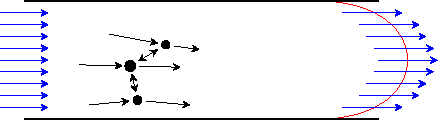
\includegraphics[width=\linewidth]{figure/dispersed_flow.pdf}
    } {\raggedleft \tiny Escoamento entre placas, Hagen-Poiseuille.}
  \end{figure}
\end{frame}

\subsection{Escoamentos em Turbomáquinas}
\begin{frame}
  \frametitle{\subsecname}
  %-Este exemplo demonstra que é apropriado assumir que o escoamento no disco de uma turbomáquina é
  % bidimensional, e sem efeito da gravidade
  
  \begin{block}{Objetivos deste trabalho:}
    Estudar como partículas se comportam dentro de uma turbomáquina em funcionamento.
  \end{block}
  
  \begin{figure}
    \stackunder{
      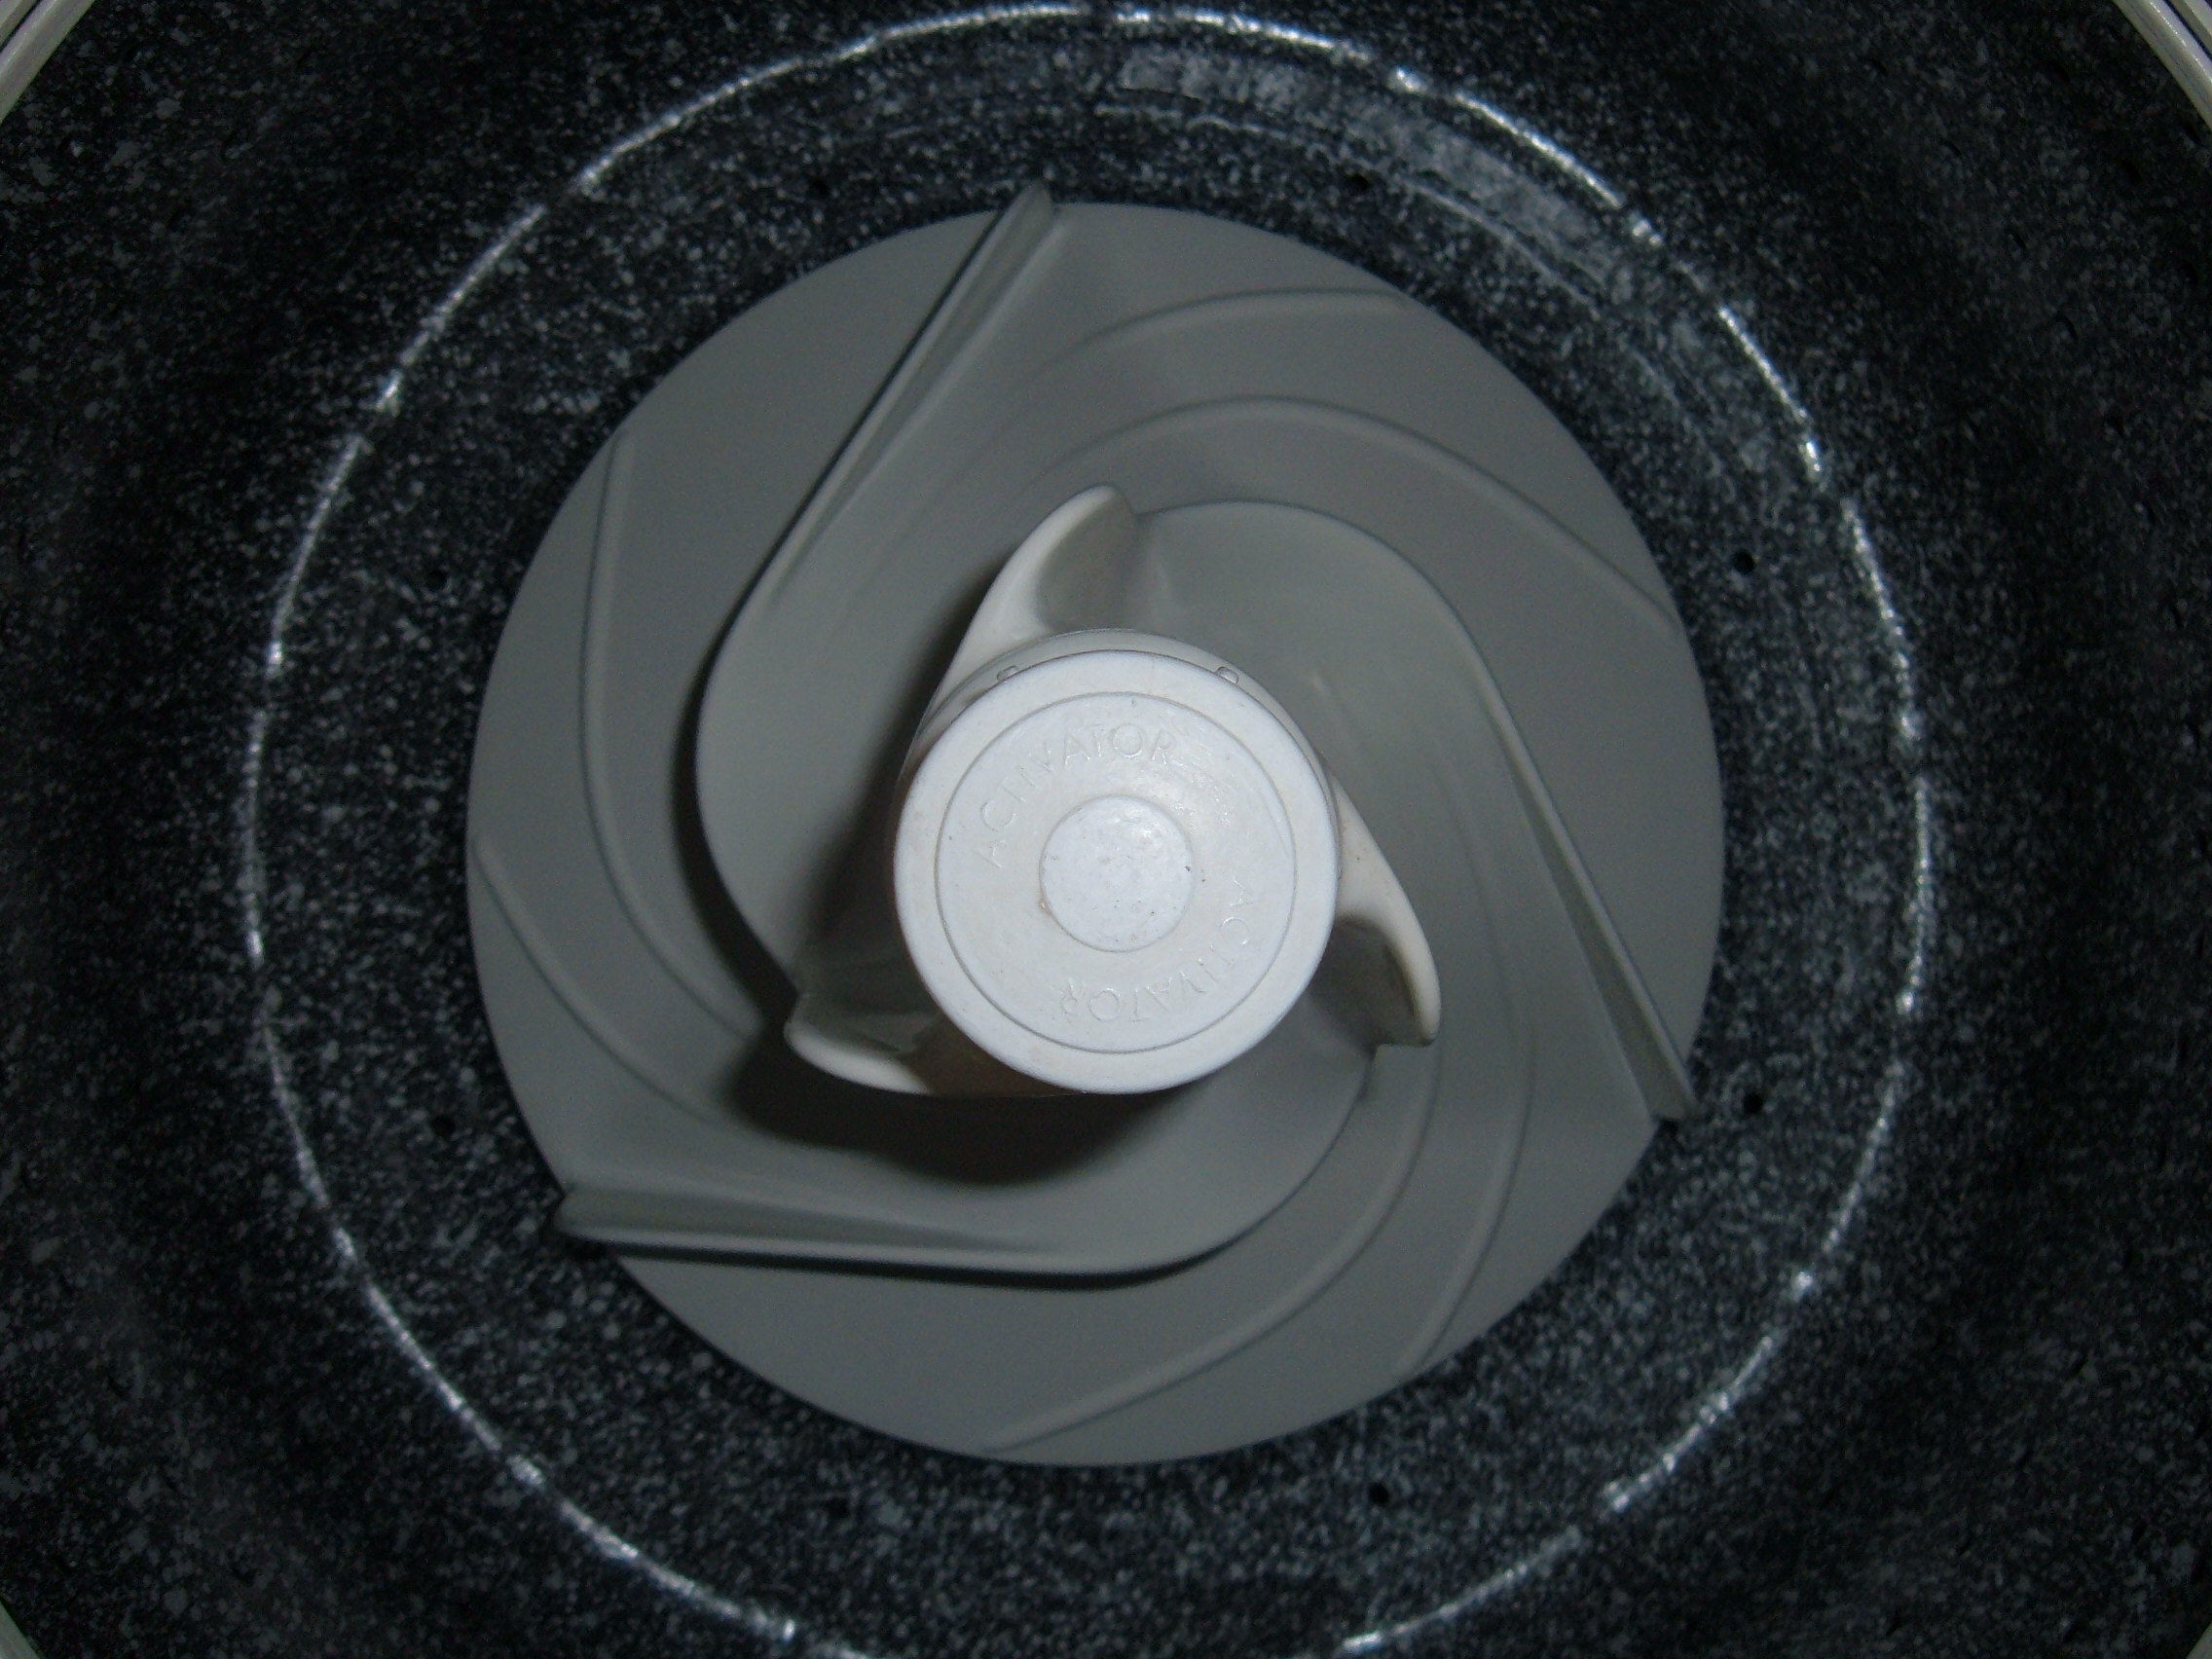
\includegraphics[width=0.6\linewidth]{figure/Washing_machine_agitator.jpg}
    } {\raggedleft \tiny Fonte:\href{https://commons.wikimedia.org/wiki/File:Washing_machine_agitator.JPG}
      {\textcopyright \ BrokenSphere / Wikimedia Commons.}}
  \end{figure}
\end{frame}

%----------------------------------------------------------------------------------------------------------------------------------------------------
\section{Equações de Governo}
%----------------------------------------------------------------------------------------------------------------------------------------------------

\subsection{Formulação Corrente-Vorticidade}
\begin{frame}
  \frametitle{\subsecname}
  %-Primeiro falaremos sobre a equação de Naiver-Stoakes e esta forma e obtida através dela
  
  \begin{block}{Hipóteses tomadas}
    \begin{itemize}
     \item Fluído incompressível
     \item Fluído newtoniano
    \end{itemize}
  \end{block}
  
  \begin{block}{Equação de Navier-Stoakes}
    \centering
    $\dfrac{\partial \vec{v}_f}{\partial t} + \vec{v}_f.\vec{\nabla}\vec{v}_f =
    -\dfrac{1}{\rho_f} \vec{\nabla}p + \dfrac{\mu_f}{\rho_f} \nabla^2\vec{v}_f + \vec{g}$
  \end{block}
  
  \begin{block}{Desvantagens}
    \begin{itemize}
     \item Requer o uso da equação auxiliar da continuidade devido a presença da pressão
     \item Acoplamento da pressão e velocidade
     \item Exige elementos de ordem elevada
    \end{itemize}
  \end{block}
\end{frame}


\begin{frame}
  \frametitle{\subsecname}
  %-Esta formulação e uma alternativa a equação de Navier-Stoakes para encontrar o campo de velocidades do escoamento
  % Desta forma, consegue-se solucionar o sistema menos complexo, pois NS exige elementos de ordem superior para garantir a converg^encia
  % Isto permite uma solução mais simples e rápida
  
  \begin{minipage}{.53\textwidth}
    \begin{block}{Equação da Vorticidade}
      \centering
      $\dfrac{\partial \vec{\omega}}{\partial t} + \vec{v}_f.\vec{\nabla}\vec{\omega} = \dfrac{\mu_f}{\rho_f} \nabla^2 \vec{\omega}$
    \end{block}
    
    \begin{block}{Equação da Corrente}
      \centering
      $\nabla^2\psi = -\omega_z$
    \end{block}
  \end{minipage}
  \hfill
  \begin{minipage}{.41\textwidth}
    \begin{block}{Equações Auxiliares}
      \vspace*{-\baselineskip}\setlength\belowdisplayshortskip{0pt} % Fix display bug, empty header space
      \centering
      \begin{align*}
	\vec{v}_f &= \left(v_{f,x}\, , v_{f,y} \right)\\
	v_{f,x} &= \partfrac2{\psi}{y} \\
	v_{f,y} &= -\partfrac2{\psi}{x} \\
	\omega_z &= \partfrac2{v_{f,x}}{y} - \partfrac2{v_{f,y}}{x} 
      \end{align*}
    \end{block}
  \end{minipage}
\end{frame}

%----------------------------------------------------------------------------------------------------------------------------------------------------
\subsection{Equação de Basset–Boussinesq–Oseen (BBO)}
\begin{frame}
  \frametitle{\subsecname}
  %-Mencionar diferenças entre a equação de Reynolds da partícula e o normal
  
%   \begin{block}{}
    Equação que representa as forças exercidas sobre as partículas.
    Sua expressão é a soma das forças separadamente.
%   \end{block}
  
  \begin{block}{Equação de Basset–Boussinesq–Oseen}
    \centering
    $\vec{F}_{p} = \sum\vec{F} = \vec{F}_{grav} + \vec{F}_{drag} + \vec{F}_{lift} + \vec{F}_{mass}$
  \end{block}
  
  \begin{minipage}{.50\textwidth}
    \begin{block}{Restrição}
      A equação BBO é somente válida para Reynolds da partícula menores que 1.
      $Re_{p} < 1$
    \end{block}
  \end{minipage}
  \hfill
  \begin{minipage}{.46\textwidth}
    \begin{block}{Reynolds de Partícula}
      \centering
      $Re_{p} = \dfrac{\rho_p}{\mu_f} |\left(\vec{v}_{f} - \vec{v}_{p} \right)|_{max}\, d_{p}$
    \end{block}
  \end{minipage}
\end{frame}


\begin{frame}
  \frametitle{\subsecname}
  
  \begin{minipage}{.45\textwidth}
    \begin{block}{Força Gravitacional}
      \centering
      $\vec{F}_{grav} = m_p \vec{g}$
    \end{block}
    
    \begin{block}{Força de Arrasto}
      \centering
      $\vec{F}_{drag} = 3 \pi \mu_f d_p \left(\vec{v}_{f} - \vec{v}_{p} \right)$
    \end{block}
  \end{minipage}
  \hfill
  \begin{minipage}{.51\textwidth}
    \begin{block}{Força de Sustentação}
      \centering
      $\vec{F}_{lift} = 1.61 \mu_f d_p \left(\vec{v}_{f} - \vec{v}_{p} \right) \sqrt{{Re}_G}$
    \end{block}
    
    \begin{block}{Força de Massa Virtual}
      \centering
      $\vec{F}_{mass} = \dfrac{1}{2} \rho_f V_p \dfrac{d}{dt}\left(\vec{v}_{f} - \vec{v}_{p} \right)$
    \end{block}
  \end{minipage}
  
  \begin{block}{Reynolds de Cisalhamento}
    \centering
    $Re_G = \dfrac{\rho_f}{\mu_f} d_p^2 \nabla \vec{v}_f$
  \end{block}
\end{frame}

%----------------------------------------------------------------------------------------------------------------------------------------------------
\section{Métodos Numéricos}
%----------------------------------------------------------------------------------------------------------------------------------------------------

\subsection{Método dos Elementos Finitos}
\begin{frame}
  \frametitle{\subsecname}
  %-
  
  \begin{block}{Domínio}
    Equações são definidas em um domínio $\Omega$ com contorno $\Gamma$.
  \end{block}
    
  \begin{minipage}{.61\textwidth}
    \begin{block}{Forma forte com as funções peso}
      \vspace*{-\baselineskip}\setlength\belowdisplayshortskip{0pt} % Fix display bug, empty header space
      \begin{equation*}
	\int_{\Omega} \left(
	\dfrac{\partial \vec{\omega}}{\partial t} +
	\vec{v}_f.\vec{\nabla}\vec{\omega} -
	\dfrac{\mu_f}{\rho_f} \nabla^2 \vec{\omega}
	\right).\vec{\delta} d\Omega = 0
      \end{equation*}
      \vspace*{-\baselineskip}\setlength\belowdisplayshortskip{3pt} % Fix display bug, empty header space
      \vspace{5pt}
      \begin{equation*}
	\int_{\Omega} \left(
	\nabla^2\psi +
	\omega_z
	\right).\vec{\phi} d\Omega = 0
      \end{equation*}
      \vspace{3pt}
      \begin{equation*}
	\int_{\Omega} \left(
	\vec{v}_f - \left(\dfrac{\partial \psi}{\partial y},
	-\dfrac{\partial \psi}{\partial x} \right)
	\right).\vec{\xi} d\Omega = 0
      \end{equation*}
    \end{block}
  \end{minipage}
  \hfill
  \begin{minipage}{.34\textwidth}
    \begin{block}{Condições de contorno}
      \vspace*{-\baselineskip}\setlength\belowdisplayshortskip{0pt} % Fix display bug, empty header space
      \begin{align*}
	\omega &= \omega_{\Gamma} \text{ em } \Gamma \\
	\psi &= \psi_{\Gamma} \text{ em } \Gamma \\
	\vec{v}_f &= \vec{v}_{f\Gamma} \text{ em } \Gamma 
      \end{align*}
    \end{block}
  \end{minipage}
  
  \vspace{5pt}
  $\vec{\delta}$, $\vec{\phi}$ e $\vec{\xi}$ são as funções de peso de cada equação.
\end{frame}


\begin{frame}
  \frametitle{\subsecname}
  %-Simplificação do omega_z para omega
  
  \begin{block}{Forma fraca}
      \vspace*{-\baselineskip}\setlength\belowdisplayshortskip{0pt} % Fix display bug, empty header space
    \begin{align*}
      m_1 \left(\dfrac{\partial \vec{\omega}}{\partial t}, \delta\right) +
      g_1 (\vec{v}_f, \vec{\delta}) + 
      \dfrac{\mu_f}{\rho_f} k_1 (\vec{\omega}, \vec{\delta}) &=0\\
      -k_2 (\psi, \vec{\phi}) +
      m_2 (\omega_z, \vec{\phi}) &= 0 \\
      m_3 (\vec{v}_f, \vec{\xi}) - 
      g_3 (\psi, \vec{\xi}) &=0
    \end{align*}
  \end{block}
  
  \fontsize{8}{7.2}\selectfont
  \begin{minipage}{.48\textwidth}
    \begin{block}{Onde:}
    \begin{equation*}
	m_1 \left(\dfrac{\partial \vec{\omega}}{\partial t}, \delta\right) =
	\int_{\Omega}
	\dfrac{\partial \vec{\omega}}{\partial t}
	.\vec{\delta} d\Omega
      \end{equation*}
      \begin{equation*}
	g_1 (\vec{v}_f, \vec{\delta}) =
	\int_{\Omega}
	\vec{v}_f.\vec{\nabla}\vec{\omega}
	.\vec{\delta} d\Omega
      \end{equation*}
%       \vspace{5pt}
      \begin{equation*}
	k_1 (\vec{\omega}, \vec{\delta}) =
	\int_{\Omega}
	\vec{\nabla}\vec{\omega}.\vec{\nabla}
	\vec{\delta} d\Omega
      \end{equation*}
    \end{block}
  \end{minipage}
  \hfill
  \begin{minipage}{.48\textwidth}
    \begin{block}{}
      \begin{equation*}
	k_2 (\psi, \vec{\phi}) =
	\int_{\Omega}
	\vec{\nabla}\psi.\vec{\nabla}
	\vec{\phi} d\Omega
      \end{equation*}
      \begin{equation*}
	m_2 (\omega_z, \vec{\phi}) =
	\int_{\Omega}
	\omega_z
	.\vec{\phi} d\Omega
      \end{equation*}
      \begin{equation*}
	m_3 (\vec{v}_f, \vec{\xi}) =
	\int_{\Omega}
	\vec{v}_f
	.\vec{\xi} d\Omega
      \end{equation*}
      \begin{equation*}
	g_3 (\psi, \vec{\xi}) =
	\int_{\Omega}
	\left(\dfrac{\partial \psi}{\partial y},
	-\dfrac{\partial \psi}{\partial x} \right)
	.\vec{\xi} d\Omega
      \end{equation*}
    \end{block}
  \end{minipage}
\end{frame}

%----------------------------------------------------------------------------------------------------------------------------------------------------
\subsection{Discretizações dos Modelos}
\begin{frame}
  \frametitle{Discretização do Modelo de Escoamentos}
  %-
  
  \begin{block}{Formulação de Galerkin}
    Funções de peso são definidas com valor igual às funções interpoladoras.
    
    \begin{minipage}{.45\textwidth}
      \vspace*{-\baselineskip}\setlength\belowdisplayshortskip{0pt} % Fix display bug, empty header space
      \begin{align*}
	\omega(\vec{x}, t) &= \sum_{i=1}^{n_p} \omega_i(t) N_i(\vec{x}) \\
	\psi(\vec{x}, t) &= \sum_{i=1}^{n_p} \psi_i(t) N_i(\vec{x}) \\
	v_{f,x}(\vec{x}, t) &= \sum_{i=1}^{n_p} v_{f,x,i}(t) N_i(\vec{x}) \\
	v_{f,y}(\vec{x}, t) &= \sum_{i=1}^{n_p} v_{f,y,i}(t) N_i(\vec{x}) 
      \end{align*}
    \end{minipage}
    \hfill
    \begin{minipage}{.45\textwidth}
      \vspace*{-\baselineskip}\setlength\belowdisplayshortskip{0pt} % Fix display bug, empty header space
      \begin{align*}
	\delta(\vec{x}, t) &= \sum_{j=1}^{n_p} \delta_i(t) N_j(\vec{x}) \\
	\phi(\vec{x}, t) &= \sum_{j=1}^{n_p} \phi_i(t) N_j(\vec{x}) \\
	\xi(\vec{x}, t) &= \sum_{j=1}^{n_p} \xi_i(t) N_j(\vec{x})
      \end{align*}
    \end{minipage}
  \end{block}
\end{frame}

\begin{frame}
  \frametitle{Discretização do Modelo de Escoamentos}
  %-
  
  \begin{block}{Função de Aproximação}
    $N(x)$ é a função de aproximação de cada elemento:
    \begin{equation*}
      N_{i}(\vec{x}) = [N_{1}(\vec{x}), \ldots, N_{n_p}(\vec{x})]
    \end{equation*}
  \end{block}
  
  \begin{block}{Matrizes locais dos elementos}
    Surgem os termos locais, para cada elemento $e$:
    \begin{minipage}{.45\textwidth}
      \vspace*{-\baselineskip}\setlength\belowdisplayshortskip{0pt} % Fix display bug, empty header space
      \vspace{5pt}
      \begin{align*}
	\mathbf{m^e} &=
	\int_{\Omega^e}
	N_i^e N_j^e
	d\Omega^e \\
	\mathbf{g_x^e} &=
	\int_{\Omega^e}
	\dfrac{\partial N_i^e}{\partial x}
	N_j^e
	d\Omega^e \\
	\mathbf{g_y^e} &=
	\int_{\Omega^e}
	\dfrac{\partial N_i^e}{\partial y}
	N_j^e
	d\Omega^e
      \end{align*}
    \end{minipage}
    \hfill
    \begin{minipage}{.45\textwidth}
      \vspace*{-\baselineskip}\setlength\belowdisplayshortskip{0pt} % Fix display bug, empty header space
      \begin{align*}
	\mathbf{k_{xx}^e} &=
	\int_{\Omega^e}
	\dfrac{\partial N_i^e}{\partial x}
	\dfrac{\partial N_j^e}{\partial x}
	d\Omega^e \\
	\mathbf{k_{yy}^e} &=
	\int_{\Omega^e}
	\dfrac{\partial N_i^e}{\partial y}
	\dfrac{\partial N_j^e}{\partial y}
	d\Omega^e
      \end{align*}
    \end{minipage}
  \end{block}
\end{frame}
  
\begin{frame}
  \frametitle{Discretização do Modelo de Escoamentos}
  %-
  
  \begin{block}{Discretização no tempo}
    Para os termos temporais é utilizada o Método de Diferenças Finitas:
    \begin{equation*}
      \dfrac{\partial \omega}{\partial t} \approx
      \frac{
	  \omega(t + dt) -
	  \omega(t)
      }{dt}
      =
      \frac{
	  \omega^{t_{n+1}} -
	  \omega^{t_{n}}
      }{dt}
    \end{equation*}
  \end{block}
  
  \begin{block}{Equações na forma global}
    \begin{equation*}
      \left(
	  \mathbf{M} v_{f,x}^{t_{n}} \mathbf{G_x} + v_{f,y}^{t_{n}} \mathbf{G_y} + \dfrac{\mu_f}{\rho_f}
	  \left( \mathbf{K_{xx}} + \mathbf{K_{yy}} \right)
      \right)
      \omega^{t_{n+1}} = \mathbf{M} \omega^{t_{n}}
      \label{last_w}
    \end{equation*}
    \begin{equation*}
      \left( \mathbf{K_{xx}} + \mathbf{K_{yy}} \right)
      \psi = \mathbf{M} \omega^{t_{n+1}}
      \label{last_psi}
    \end{equation*}
    \begin{equation*}
      \mathbf{M} v_{f,x}^{t_{n}} \omega^{t_{n+1}} =
      \mathbf{G_y} \psi
      \label{last_vx}
    \end{equation*}
    \begin{equation*}
      \mathbf{M} v_{f,y}^{t_{n}} \omega^{t_{n+1}} = 
      -\mathbf{G_x} \psi
      \label{last_vy}
    \end{equation*}
  \end{block}
\end{frame}

%----------------------------------------------------------------------------------------------------------------------------------------------------
\subsection*{Discretização do Modelo de Partículas}
\begin{frame}
  \frametitle{\subsecname}
  %-V grande e o volume da partícula
  
  \begin{block}{Equações das forças nas partículas}
      \vspace*{-\baselineskip}\setlength\belowdisplayshortskip{0pt} % Fix display bug, empty header space
      \begin{align*}
	\vec{F}_{grav}^{t_n} &= m_p \vec{g} \\
	\vec{F}_{drag}^{t_n} &= 3 \pi \mu_f d_p \left(\vec{v}_{f}^{\,t_n} - \vec{v}_{p}^{\,t_{n-1}} \right) \\
	\vec{F}_{lift}^{t_n}\ \ &= 1.61 \mu_f d_p \left(\vec{v}_{f}^{\,t_n} - \vec{v}_{p}^{\,t_{n-1}} \right) \sqrt{{Re}_G^{t_n}} \\
	\vec{F}_{mass}^{t_n} &= \dfrac{1}{2} \rho_f V_p \dfrac{\left(\vec{v}_{f}^{\,t_n} - \vec{v}_{p}^{\,t_{n-1}}\right) -
	\left(\vec{v}_{f}^{\,t_{n-1}} - \vec{v}_{p}^{\,t_{n-2}} \right)}{dt}
      \end{align*}
  \end{block}

  \begin{block}{Reynolds específicos}
    \begin{minipage}{.35\textwidth}
      \vspace*{-\baselineskip}\setlength\belowdisplayshortskip{0pt} % Fix display bug, empty header space
      \begin{equation*}
	  Re_{p}^{t_n} = \dfrac{\rho_p}{\mu_f} d_{p} \left|\vec{v}_{f}^{\,t_n} - \vec{v}_{p}^{\,t_{n-1}} \right|_{max}
      \end{equation*}
    \end{minipage}
%     \hfill
    \hspace{5pt}
    \begin{minipage}{.55\textwidth}
      \begin{equation*}
	  Re_G^{t_n} = \dfrac{d_p^2 \rho_f}{\mu_f} \left( \dfrac{d\vec{v}_f}{d\vec{r}} \right)^{t_n}
      \end{equation*}
    \end{minipage}
  \end{block}
\end{frame}

%----------------------------------------------------------------------------------------------------------------------------------------------------
\subsection{Definição das Matrizes}
\begin{frame}
  \frametitle{Matrizes dos Elementos Triangulares}
  %-
  
  \fontsize{7.5}{7.2}\selectfont
  \begin{minipage}{.4\textwidth}
    \centering
    \stackunder{
      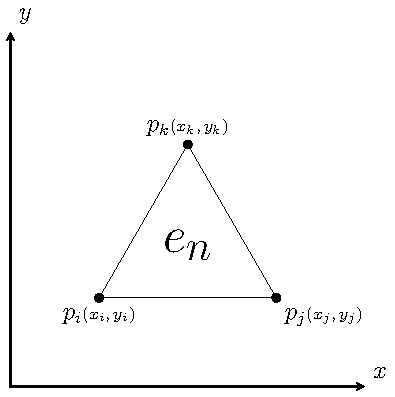
\includegraphics[width=\linewidth]{figure/element_detailed.pdf}
    } {\raggedleft \tiny Elemento triangular linear.}
  \end{minipage}
  \hfill
  \begin{minipage}{.56\textwidth}
    \begin{block}{Coordenadas relativas}
      \vspace*{-\baselineskip}\setlength\belowdisplayshortskip{0pt} % Fix display bug, empty header space
      \centering
      \begin{equation*}
      \mathbf{b} \left\{
	\begin{align*}
	  &b_i = y_j - y_k \\
	  &b_j = y_k - y_i \\
	  &b_k = y_i - y_j
	\end{align*} \right.\qquad
      \mathbf{c} \left\{
	\begin{align*}
	  &c_i = x_k - x_j \\
	  &c_j = x_i - x_k \\
	  &c_k = x_j - x_i
	\end{align*} \right.
      \end{equation*}
    \end{block}
    
    \begin{block}{Matrizes de Gradiente}
      \begin{minipage}{.48\textwidth}
	$\mathbf{g_x^e} =
	\dfrac{1}{6}
	\begin{bmatrix} 
	  b_i & b_j & b_k \\
	  b_i & b_j & b_k \\
	  b_i & b_j & b_k
	\end{bmatrix}$
      \end{minipage}
      \hfill
      \begin{minipage}{.48\textwidth}
	$\mathbf{g_y^e} =
	\dfrac{1}{6}
	\begin{bmatrix} 
	  c_i & c_j & c_k \\
	  c_i & c_j & c_k \\
	  c_i & c_j & c_k
	\end{bmatrix} $
      \end{minipage}
    \end{block}
  \end{minipage}
  
  \begin{minipage}{.24\textwidth}
    \begin{block}{Matriz de Massa}
      $\mathbf{m^e} =
      \dfrac{A^e}{12}
      \begin{bmatrix} 
	  2 & 1 & 1 \\
	  1 & 2 & 1 \\
	  1 & 1 & 2
      \end{bmatrix}$
    \end{block}
  \end{minipage}
  \hfill
  \begin{minipage}{.72\textwidth}
    \begin{block}{Matrizes de Rigidez}
      \begin{minipage}{.48\textwidth}
	$\mathbf{k_{xx}^e} =
	\dfrac{t_h}{4A}
	\begin{bmatrix} 
	    b_i b_i & b_j b_i & b_k b_i \\
	    b_i b_j & b_j b_j & b_k b_j \\
	    b_i b_k & b_j b_k & b_k b_k
	\end{bmatrix} $
      \end{minipage}
      \hfill
      \begin{minipage}{.48\textwidth}
	$\mathbf{k_{yy}^e} =
	\dfrac{t_h}{4A}
	\begin{bmatrix} 
	    c_i c_i & c_j c_i & c_k c_i \\
	    c_i c_j & c_j c_j & c_k c_j \\
	    c_i c_k & c_j c_k & c_k c_k
	\end{bmatrix}$
      \end{minipage}
    \end{block}
  \end{minipage}
\end{frame}

%----------------------------------------------------------------------------------------------------------------------------------------------------
\section{Código}
%----------------------------------------------------------------------------------------------------------------------------------------------------
\subsection{Montagem das Matrizes Globais}
\begin{frame}[fragile]
  \frametitle{\subsecname}
  %-
  
  \begin{block}{Algoritmo de montagem}
  \fontsize{6pt}{7.2}\selectfont
  \centering
    $
    \mathbf{m}_{e_n}
    =
    \begin{bmatrix}
      m_{ii} & m_{ij} & m_{ik} \\
      m_{ji} & m_{jj} & m_{jk} \\
      m_{ki} & m_{kj} & m_{kk}
    \end{bmatrix}
    \xrightarrow[\parbox{0.7cm}{l=i,j,k q=i,j,k}]{\text{loop}}
    \mathbf{M}
    =
    \begin{bmatrix}
      M_{0,0} & M_{0,1} & \ldots & M_{0,n_p} \\
      M_{1,0} & \ddots & & M_{1,n_p} \\
      \vdots & & M_{l,q} + m_{l,q} & \vdots \\
      M_{n_p, 0} & & & M_{n_p,n_p}
    \end{bmatrix}
    $
    
    \begin{verbatim}
# Loop em cada elemento na lista da malha
for elem in malha.ien:
    x = malha.x[elem] # = [x_i, x_j, x_k]
    y = malha.y[elem] # = [y_i, y_j, y_k]

    # Criação das matrizes locais
    ...

    # Registro das matrizes locais nas matrizes globais
    for i in range(3):
        for j in range(3):
            kx_global[elem[i], elem[j]] += k_x[i][j]
            ky_global[elem[i], elem[j]] += k_y[i][j]
            m_global[elem[i], elem[j]] += m[i][j]
            gx_global[elem[i], elem[j]] += g_x[i][j]
            gy_global[elem[i], elem[j]] += g_y[i][j]
    \end{verbatim}
  \end{block}
\end{frame}

%----------------------------------------------------------------------------------------------------------------------------------------------------
\subsection{Estrutura de Uso da Biblioteca}
\begin{frame}[fragile]
  \frametitle{\subsecname}
  %-Criação da malha inclue declarar as partículas
  
  \begin{figure}
    \stackunder{
      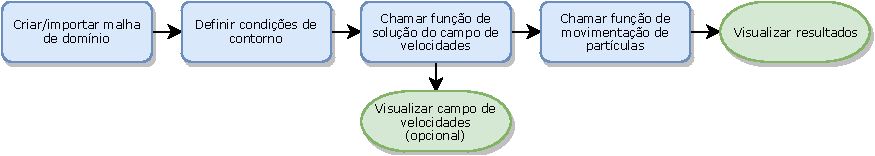
\includegraphics[width=\linewidth]{figure/TCC_Algorithm-Page-1.pdf}
    } {\raggedleft \tiny Fluxograma da lógica de uso da biblioteca pelo usuário.}
  \end{figure}
  
  
  \fontsize{5pt}{7.2}\selectfont
  \begin{minipage}{.48\textwidth}
  \begin{block}{Exemplo de uso da biblioteca}
    \begin{verbatim}
# Importação da biblioteca
import TccLib

# Importação da malha ou coordenadas de uma nova
malha = TccLib.Mesh("arquivo_da_malha.msh")
# ou malha = TccLib.Mesh([coordenadas (x, y)]

# Adição de partículas
malha.add_particle(propriedades da partícula)
    \end{verbatim}
  \end{block}
  \end{minipage}
  \hfill
  \begin{minipage}{.48\textwidth}
  \begin{block}{}
    \begin{verbatim}
# Definição das condições de contorno
malha.new_boundary_condition("nome da propriedade",
                [índices dos nós],
                [valor da condição no nó],
                [1 para Dirichlet ou 0 para Neumann])

# Chamada para a função de solução
v_x, v_y = TccLib.solve_velocity_field(malha)

# Loop de movimentação das partículas
for t in time_list:
    TccLib.move_particles(malha, (v_x, v_y))
    \end{verbatim}
  \end{block}
  \end{minipage}
\end{frame}

%----------------------------------------------------------------------------------------------------------------------------------------------------
\subsection{Estrutura de Solução}
\begin{frame}
  \frametitle{\subsecname}
  %-
  
  \begin{minipage}{.48\textwidth}
%     \centering
    \begin{figure}
      \stackunder{
	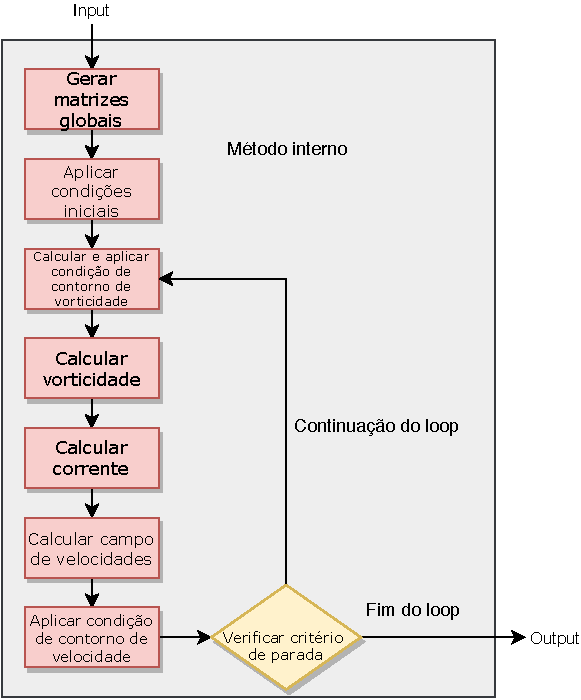
\includegraphics[height=0.7\textheight]{figure/TCC_Algorithm-Page-2.pdf}
      } {\raggedleft \tiny Algoritmo de solução do sistema de corrente-vorticidade.}
    \end{figure}
  \end{minipage}
  \hfill
  \begin{minipage}{.48\textwidth}
    \begin{figure}
      \stackunder{
	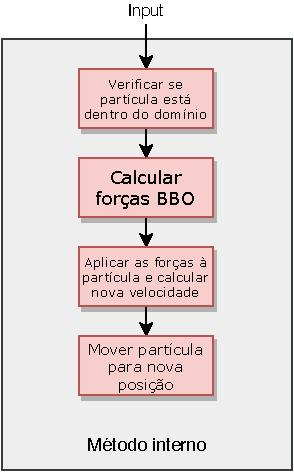
\includegraphics[height=0.7\textheight]{figure/TCC_Algorithm-Page-3.pdf}
      } {\raggedleft \tiny Algoritmo de solução da posição das partículas.}
    \end{figure}
  \end{minipage}
\end{frame}

%----------------------------------------------------------------------------------------------------------------------------------------------------
\section{Validações e Resultados}
%----------------------------------------------------------------------------------------------------------------------------------------------------
\subsection{Validações}
\begin{frame}
  \frametitle{Configurações}
  %-
  
  \begin{block}{Especificação da Máquina Utilizada}
    \begin{itemize}
      \item Dell Latitude E6410.
      \item Processador Intel® Core™ i5 CPU M 520 2.40GHz com 4 núcleos.
      \item 4Gb de memória RAM.
      \item O sistema operacional Ubuntu 16.04 LTS.
      \item Compilador Python 3.5.
    \end{itemize}
  \end{block}
  
  \begin{block}{Especificação da Máquina Utilizada}
    Foram inseridas 5 partículas igualmente espaçadas por simulação.\\
    As partículas foram colocadas próximas a entrada dos escoamentos.
  \end{block}
\end{frame}

\begin{frame}
  \frametitle{Validações de Problemas em Sólidos}
  %-Essa validação foi feita com o problema de troca térmica de laplace
  %-essas Validações permitem testar a geração de matrizes e Aplicação das condições de contorno
  
  \begin{minipage}{.48\textwidth}
    \centering
    \begin{figure}
      \stackunder{
	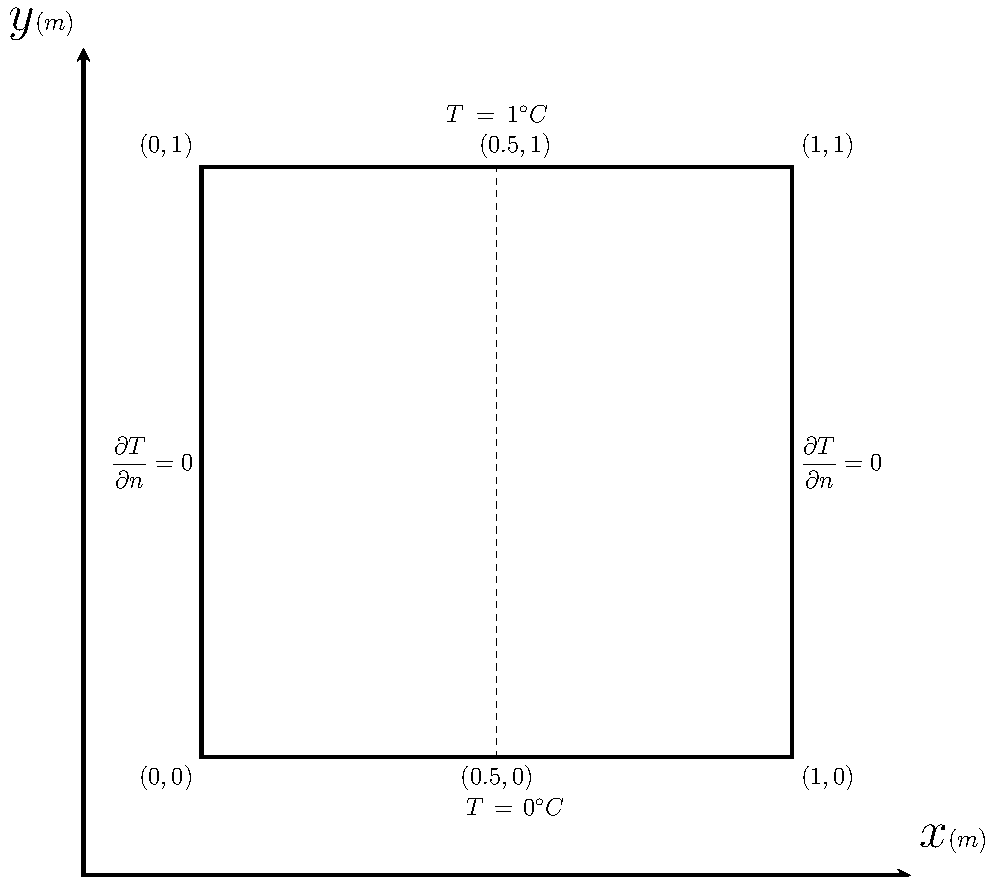
\includegraphics[height=0.38\textheight]{figure/validations/laplace_dirichlet_boundary_conditions.pdf}
      } {\raggedleft \tiny Condições de contorno em uma placa sólida.}
    \end{figure}
  \end{minipage}
  \hfill
  \begin{minipage}{.48\textwidth}
%     \centering
    \begin{figure}
      \stackunder{
	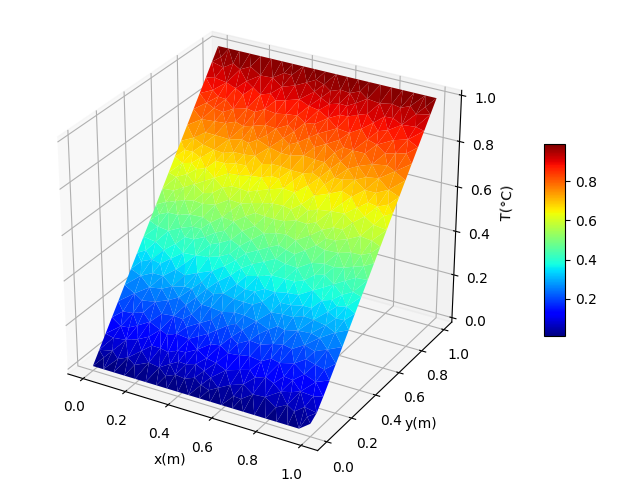
\includegraphics[height=0.38\textheight]{figure/validations/laplace_dirichlet_permanent_3d.png}
      } {\raggedleft \tiny Resultado da simulação na placa.}
    \end{figure}
  \end{minipage}
  
  \begin{minipage}{.48\textwidth}
    \begin{figure}
      \stackunder{
	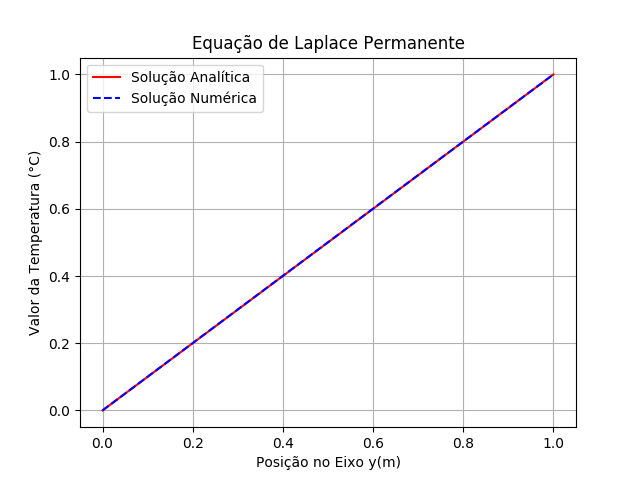
\includegraphics[height=0.38\textheight]{figure/validations/laplace_dirichlet_permanent_comparison.png}
      } {\raggedleft \tiny Comparação do resultado permanente.}
    \end{figure}
  \end{minipage}
  \hfill
  \begin{minipage}{.48\textwidth}
    \begin{figure}
      \stackunder{
	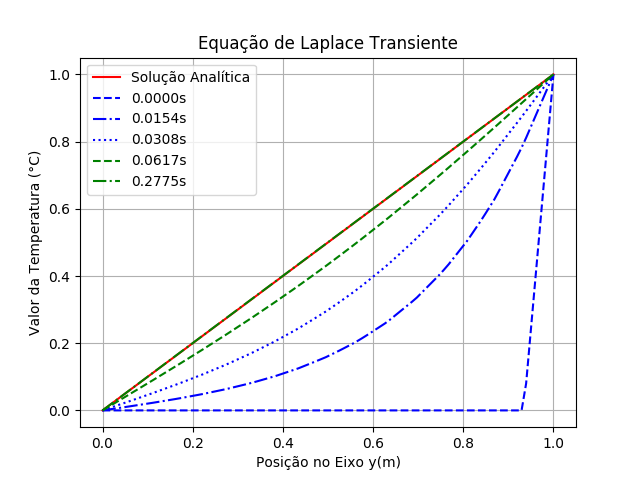
\includegraphics[height=0.38\textheight]{figure/validations/laplace_dirichlet_transient_comparison.png}
      } {\raggedleft \tiny Comparação do resultado transiente.}
    \end{figure}
  \end{minipage}
\end{frame}

\begin{frame}
  \frametitle{Validações de Problemas em Sólidos}
  %-Essa validação foi feita com o problema de troca térmica de poisson, com geração de calor
  
  \begin{minipage}{.48\textwidth}
    \centering
    \begin{figure}
      \stackunder{
	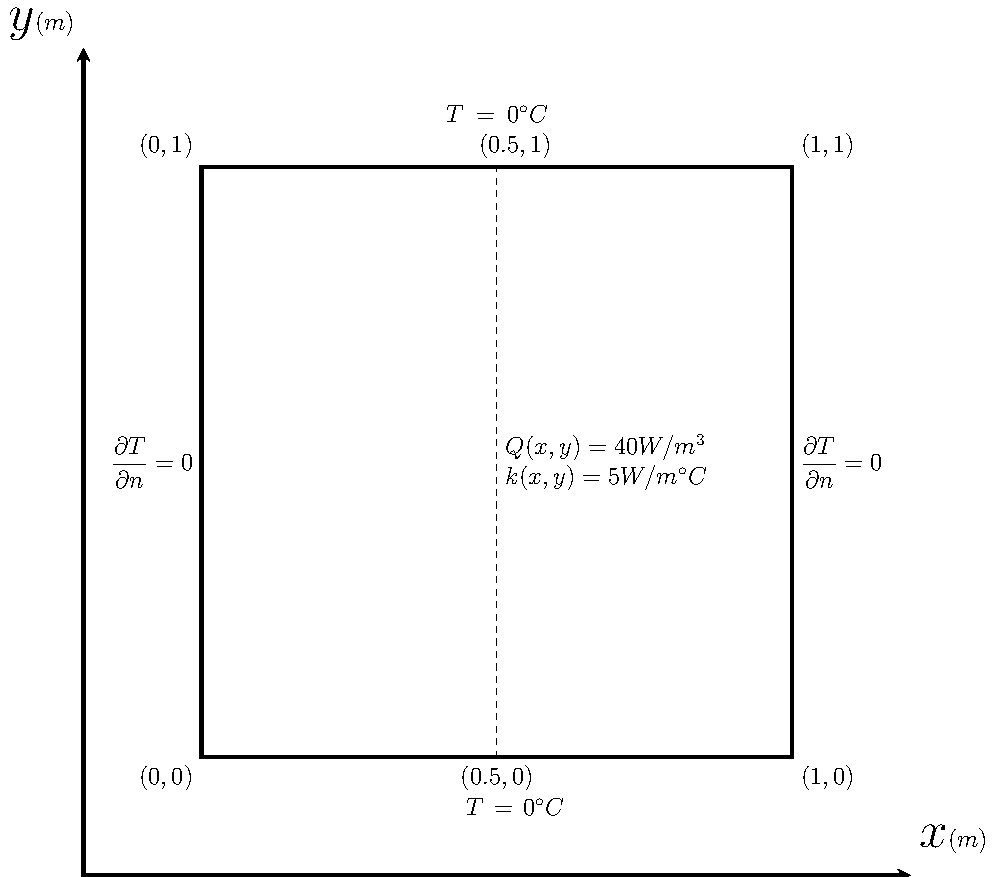
\includegraphics[height=0.38\textheight]{figure/validations/poisson_dirichlet_boundary_conditions.pdf}
      } {\raggedleft \tiny Placa com geração de calor.}
    \end{figure}
  \end{minipage}
  \hfill
  \begin{minipage}{.48\textwidth}
%     \centering
    \begin{figure}
      \stackunder{
	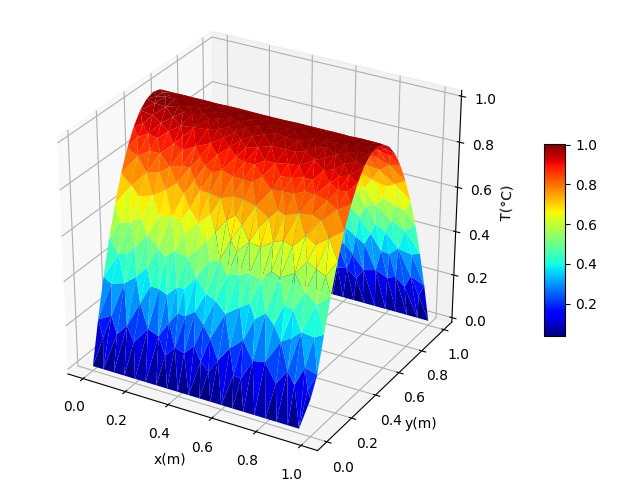
\includegraphics[height=0.38\textheight]{figure/validations/poisson_dirichlet_permanent_3d.png}
      } {\raggedleft \tiny Resultado da simulação na placa.}
    \end{figure}
  \end{minipage}
  
  \begin{minipage}{.48\textwidth}
    \begin{figure}
      \stackunder{
	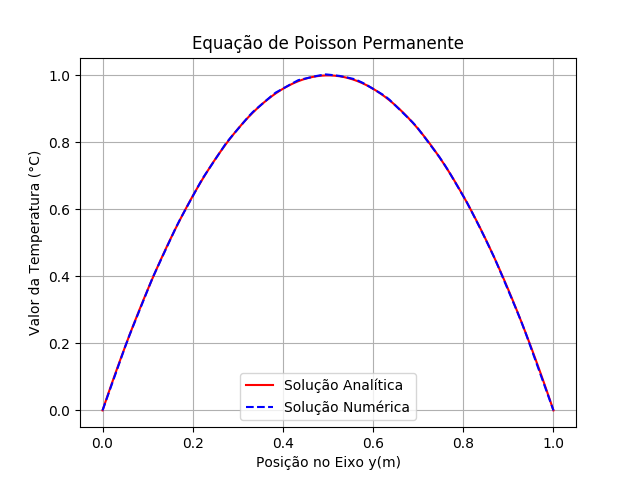
\includegraphics[height=0.38\textheight]{figure/validations/poisson_dirichlet_permanent_comparison.png}
      } {\raggedleft \tiny Comparação do resultado permanente.}
    \end{figure}
  \end{minipage}
  \hfill
  \begin{minipage}{.48\textwidth}
    \begin{figure}
      \stackunder{
	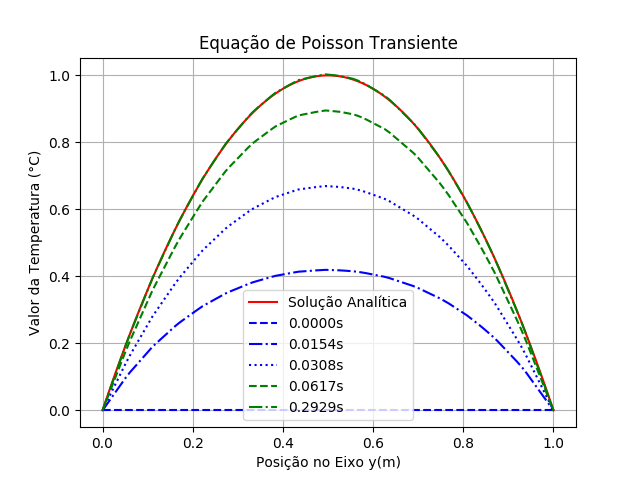
\includegraphics[height=0.38\textheight]{figure/validations/poisson_dirichlet_transient_comparison.png}
      } {\raggedleft \tiny Comparação do resultado transiente.}
    \end{figure}
  \end{minipage}
\end{frame}


\begin{frame}
  \frametitle{Validações de Problemas em Sólidos}
  %-Essa validação foi feita com o problema de troca térmica de poisson, com geração de calor e condições de contorno de Neumann
  
  \begin{minipage}{.48\textwidth}
    \centering
    \begin{figure}
      \stackunder{
	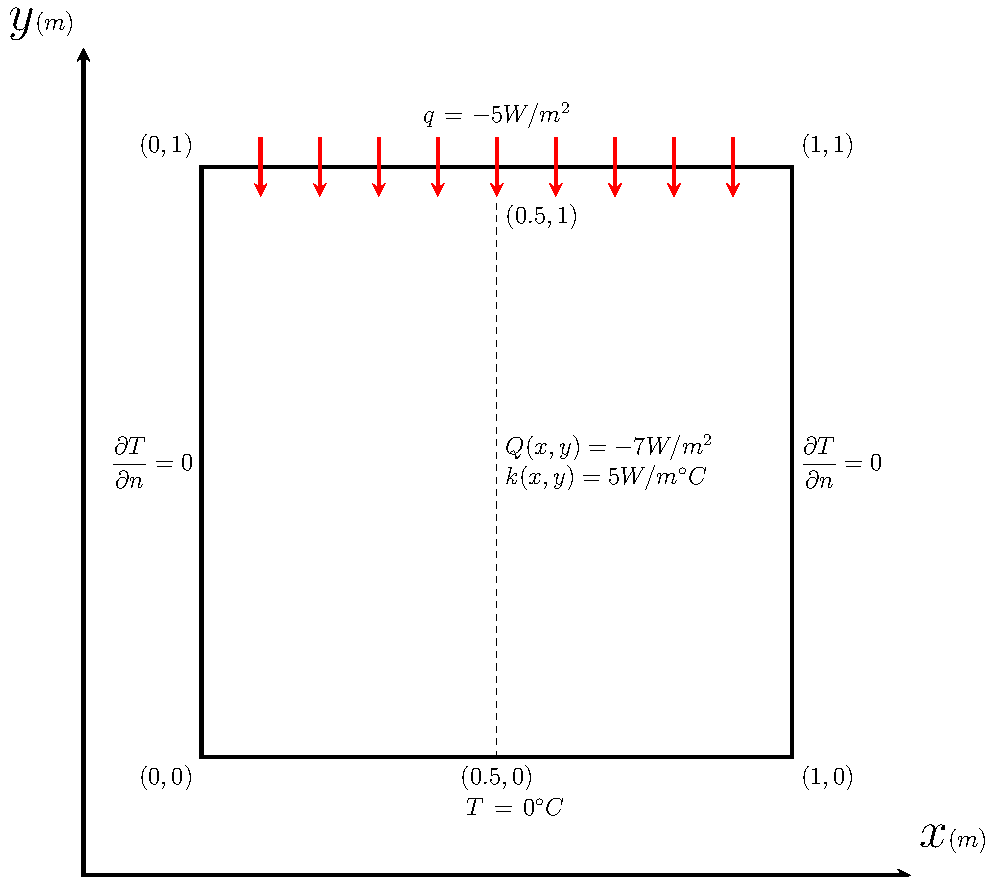
\includegraphics[height=0.38\textheight]{figure/validations/poisson_neumann_boundary_conditions.pdf}
      } {\raggedleft \tiny Placa com fluxo e geração de calor.}
    \end{figure}
  \end{minipage}
  \hfill
  \begin{minipage}{.48\textwidth}
%     \centering
    \begin{figure}
      \stackunder{
	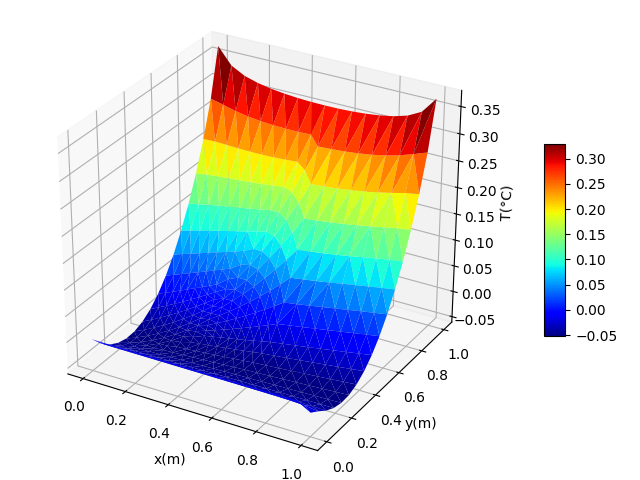
\includegraphics[height=0.38\textheight]{figure/validations/poisson_neumann_permanent_3d.png}
      } {\raggedleft \tiny Resultado da simulação na placa.}
    \end{figure}
  \end{minipage}
  
  \begin{minipage}{.48\textwidth}
    \begin{figure}
      \stackunder{
	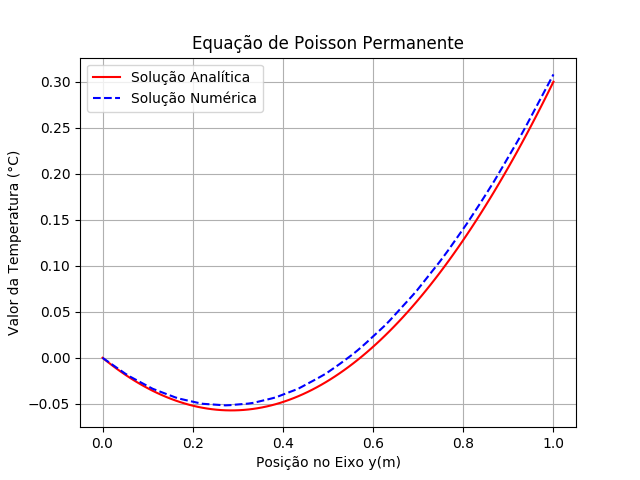
\includegraphics[height=0.38\textheight]{figure/validations/poisson_neumann_permanent_comparison.png}
      } {\raggedleft \tiny Comparação do resultado permanente.}
    \end{figure}
  \end{minipage}
  \hfill
  \begin{minipage}{.48\textwidth}
    \begin{figure}
      \stackunder{
	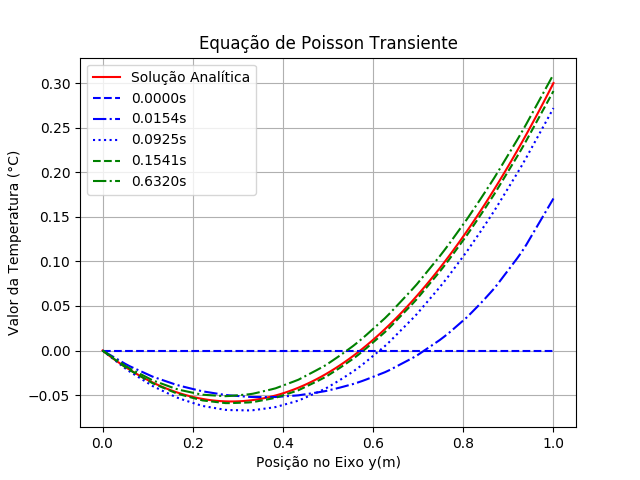
\includegraphics[height=0.38\textheight]{figure/validations/poisson_neumann_transient_comparison.png}
      } {\raggedleft \tiny Comparação do resultado transiente.}
    \end{figure}
  \end{minipage}
\end{frame}

%----------------------------------------------------------------------------------------------------------------------------------------------------
\subsection*{Validações do Modelo Corrente-Vorticidade}
\begin{frame}
  \frametitle{\subsecname}
  %-
  
  \begin{minipage}{.60\textwidth}
    \begin{figure}
      \stackunder{
	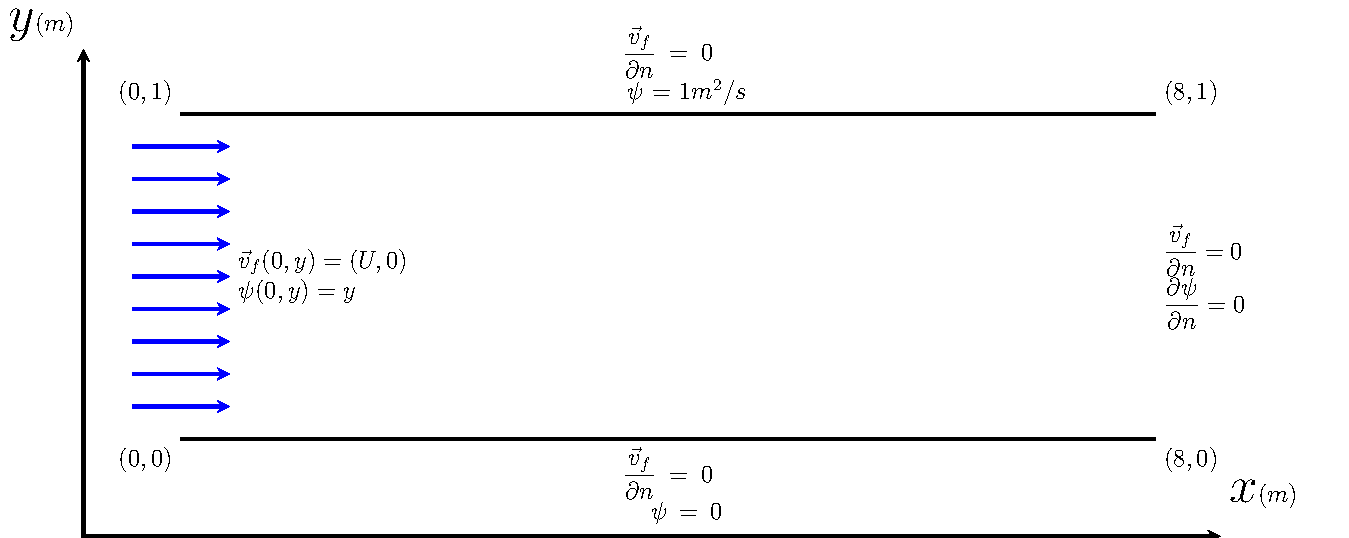
\includegraphics[height=0.32\textheight]{figure/validations/Poiseuille_boundary_conditions.pdf}
      } {\raggedleft \tiny Escoamento entre placas estacionárias (Poiseuille).}
    \end{figure}
    \vspace*{-\baselineskip}\setlength\belowdisplayshortskip{0pt} % Fix display bug, empty header space
    \begin{figure}
      \stackunder{
	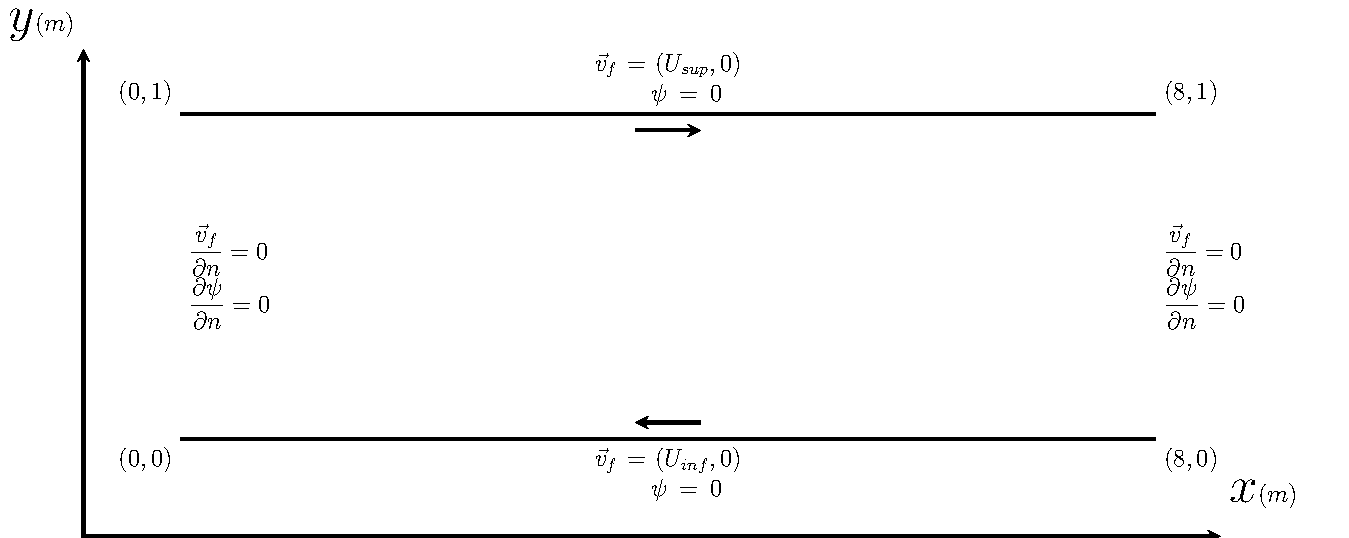
\includegraphics[height=0.32\textheight]{figure/validations/Couette_boundary_conditions.pdf}
      } {\raggedleft \tiny Escoamento entre placas em movimento (Couette).}
    \end{figure}
  \end{minipage}
  \hfill
  \begin{minipage}{.36\textwidth}
    \begin{figure}
      \stackunder{
	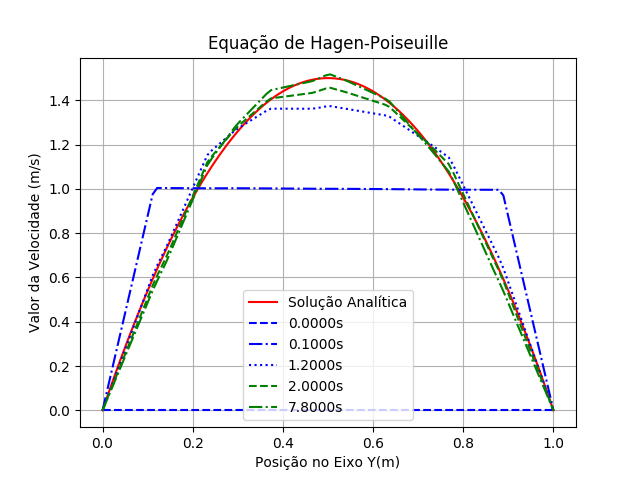
\includegraphics[height=0.32\textheight]{figure/validations/Poiseuille_validation.png}
      } {\raggedleft \tiny Comparação com solução analítica.}
    \end{figure}
    \vspace*{-\baselineskip}\setlength\belowdisplayshortskip{0pt} % Fix display bug, empty header space
    \begin{figure}
      \stackunder{
	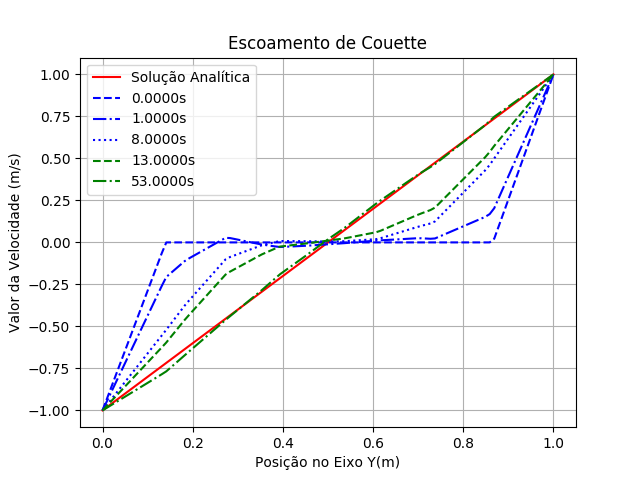
\includegraphics[height=0.32\textheight]{figure/validations/Couette_validation.png}
      } {\raggedleft \tiny Comparação com solução analítica.}
    \end{figure}
  \end{minipage}
\end{frame}

%----------------------------------------------------------------------------------------------------------------------------------------------------
\subsection*{Validações das Forças nas Partículas}
\begin{frame}
  \frametitle{\subsecname}
  %-
  
  \begin{minipage}{.48\textwidth}
    \centering
    \begin{figure}
      \stackunder{
	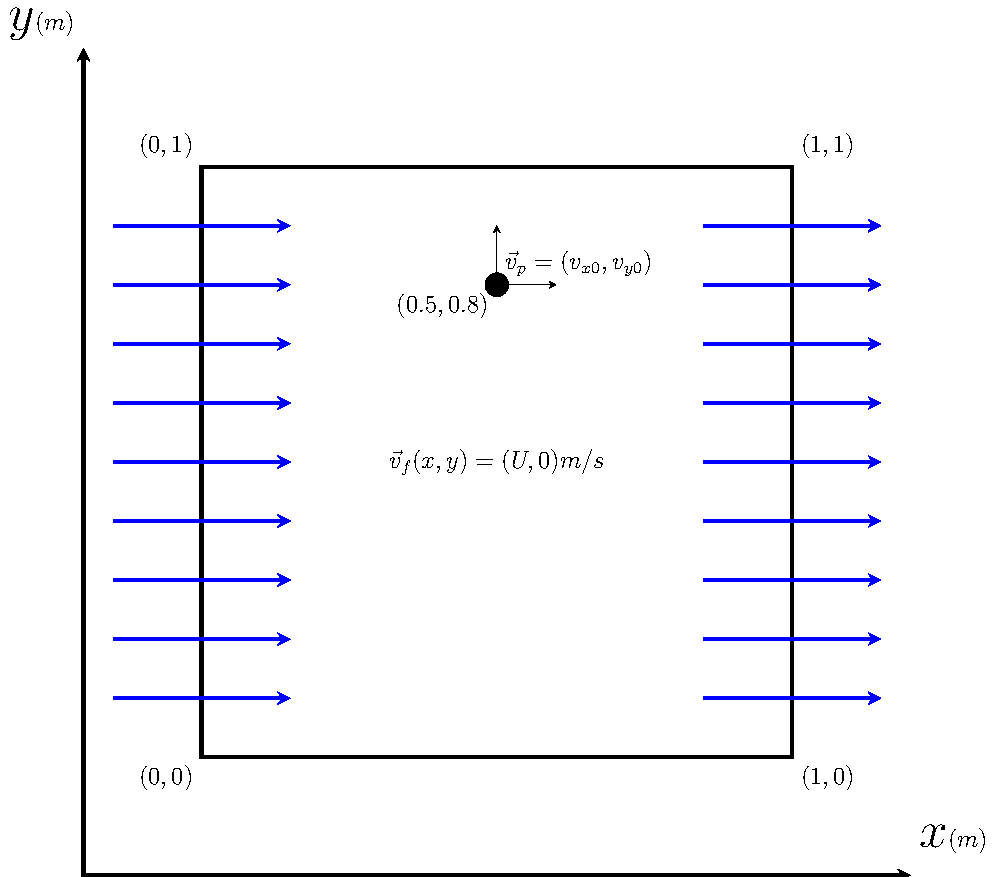
\includegraphics[height=0.38\textheight]{figure/validations/forces_boundary_conditions.pdf}
      } {\raggedleft \tiny Condições de contorno das forças indiviuais.}
    \end{figure}
  \end{minipage}
  \hfill
  \begin{minipage}{.48\textwidth}
%     \centering
    \begin{figure}
      \stackunder{
	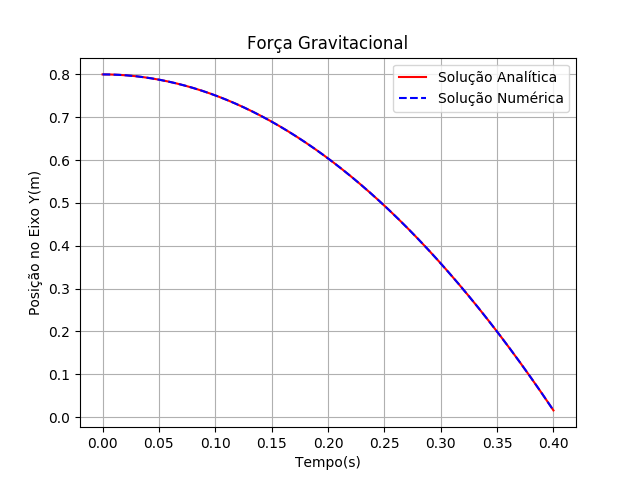
\includegraphics[height=0.38\textheight]{figure/validations/Forces_gravitational_validation.png}
      } {\raggedleft \tiny Partícula sob efeito da força gravitacional.}
    \end{figure}
  \end{minipage}
  
  \begin{minipage}{.48\textwidth}
    \begin{figure}
      \stackunder{
	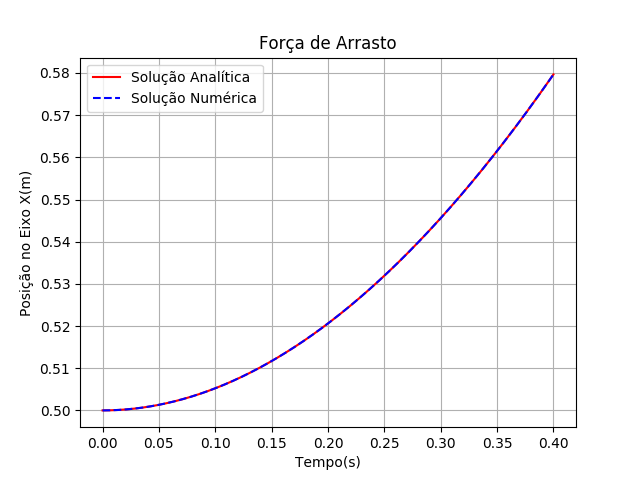
\includegraphics[height=0.38\textheight]{figure/validations/Forces_drag_validation.png}
      } {\raggedleft \tiny Partícula sob efeito da força de arrasto.}
    \end{figure}
  \end{minipage}
  \hfill
  \begin{minipage}{.48\textwidth}
    \begin{figure}
      \stackunder{
	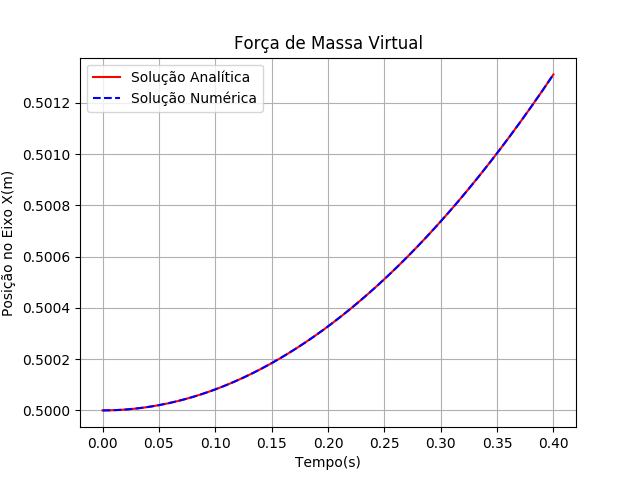
\includegraphics[height=0.38\textheight]{figure/validations/Forces_added_mass_validation.png}
      } {\raggedleft \tiny Partícula sob efeito da força de massa virtual.}
    \end{figure}
  \end{minipage}
\end{frame}

\begin{frame}
  \frametitle{\subsecname}
  %-
  
  \begin{minipage}{.48\textwidth}
    \centering
    \begin{figure}
      \stackunder{
	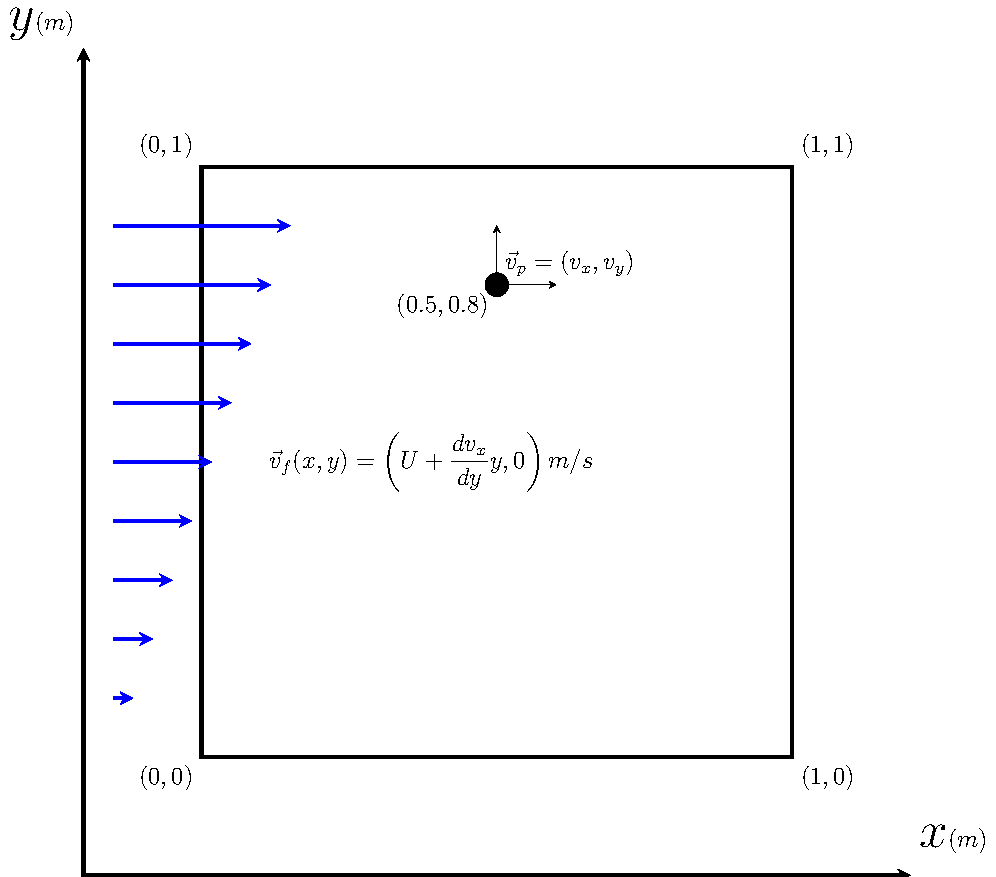
\includegraphics[height=0.48\textheight]{figure/validations/lift_boundary_conditions.pdf}
      } {\raggedleft \tiny Condições de contorno das força de sustentação.}
    \end{figure}
  \end{minipage}
  \hfill
  \begin{minipage}{.48\textwidth}
%     \centering
    \begin{figure}
      \stackunder{
	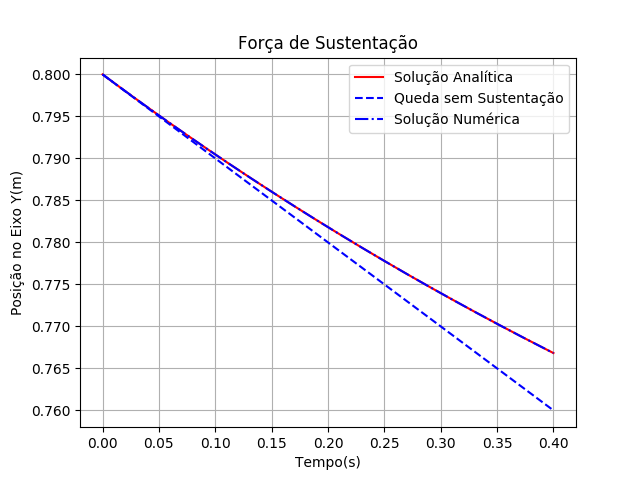
\includegraphics[height=0.48\textheight]{figure/validations/Forces_lift_validation.png}
      } {\raggedleft \tiny Partícula sob efeito da força de sustentação.}
    \end{figure}
  \end{minipage}
\end{frame}

%----------------------------------------------------------------------------------------------------------------------------------------------------
\subsection{Resultados de Simulações}
\begin{frame}
  \frametitle{Simulação em um Canal}
  %-
  
  \begin{figure}
    \stackunder{
      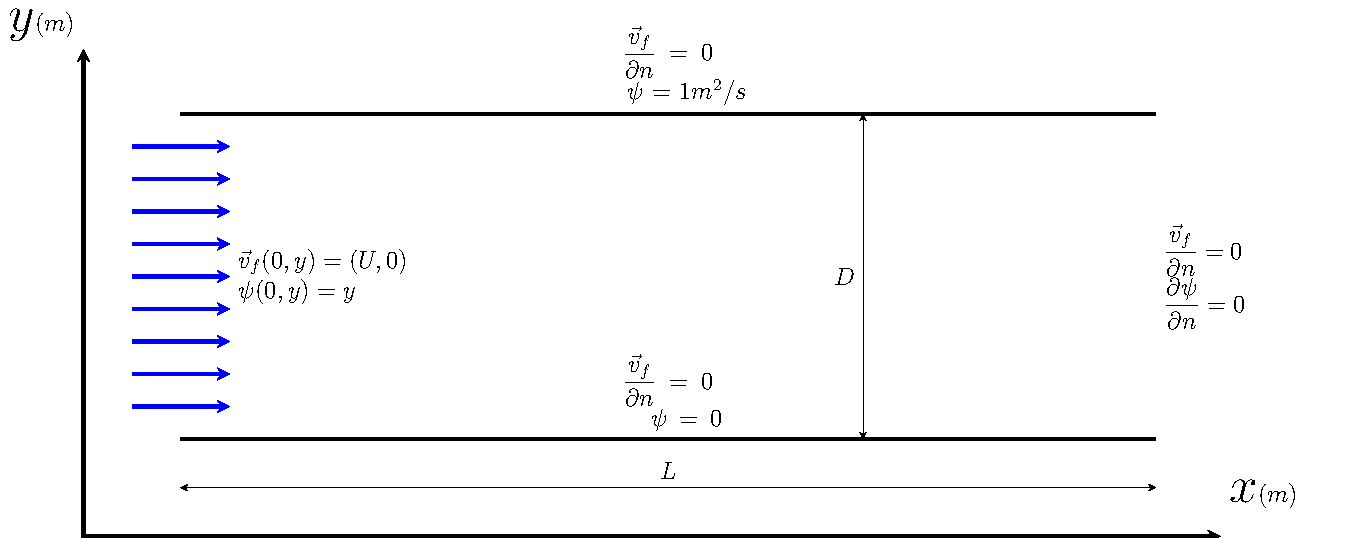
\includegraphics[height=0.38\textheight]{figure/results/Channel_boundary.pdf}
    } {\raggedleft \tiny Diagrama da simulação.}
  \end{figure}
  \begin{block}{Parâmetros}
    $L=8m$, $D=1m$, $U=1m/s$, $\mu_f=50Pa.s$, $\rho_f=50kg/m^3$, $d_p=0.001m$, $\rho_p=20000kg/m^3$.
  \end{block}
\end{frame}

\begin{frame}
  \frametitle{Simulação em um Canal}
  %-
  
  \begin{figure}
    \stackunder{
      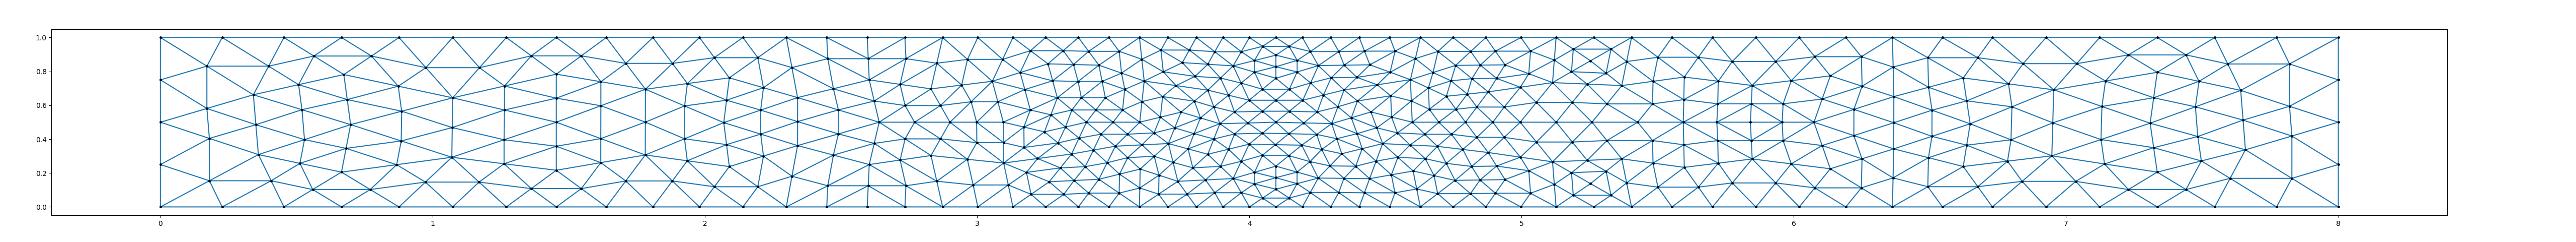
\includegraphics[width=0.98\textwidth]{figure/results/Channel_mesh.png}
    } {\raggedleft \tiny Malha do canal com 593 nós e 1072 elementos.}
  \end{figure}
  \vspace*{-\baselineskip}\setlength\belowdisplayshortskip{0pt} % Fix display bug, empty header space
  \begin{figure}
    \stackunder{
      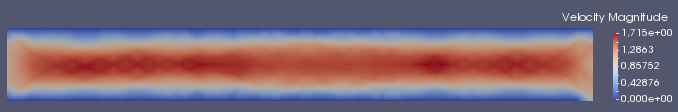
\includegraphics[width=0.98\textwidth]{figure/results/Channel_result.png}
    } {\raggedleft \tiny Campo de velocidades resultante, com $dt=0.1s$ e tempo total $t=20.0s$, realizada em torno de $1h$.}
  \end{figure}
  \vspace*{-\baselineskip}\setlength\belowdisplayshortskip{0pt} % Fix display bug, empty header space
  \begin{figure}
    \stackunder{
      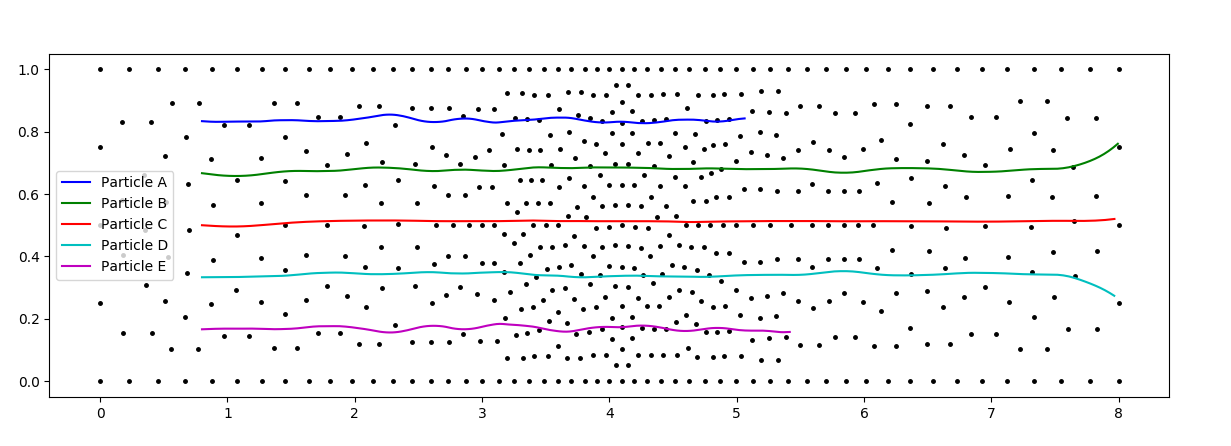
\includegraphics[height=0.28\textheight, width=0.98\textwidth]{figure/results/Channel_particle_trajectory.png}
    } {\raggedleft \tiny Percurso das partículas na simulação, com $dt=5E^{-5}$ e tempo total de $t=6.0s$, realizada em torno de $6h$.}
  \end{figure}
\end{frame}

%----------------------------------------------------------------------------------------------------------------------------------------------------
\subsection*{Simulação em um Canal com Obstáculo}
\begin{frame}
  \frametitle{\subsecname}
  %-
  
  \begin{figure}
    \stackunder{
      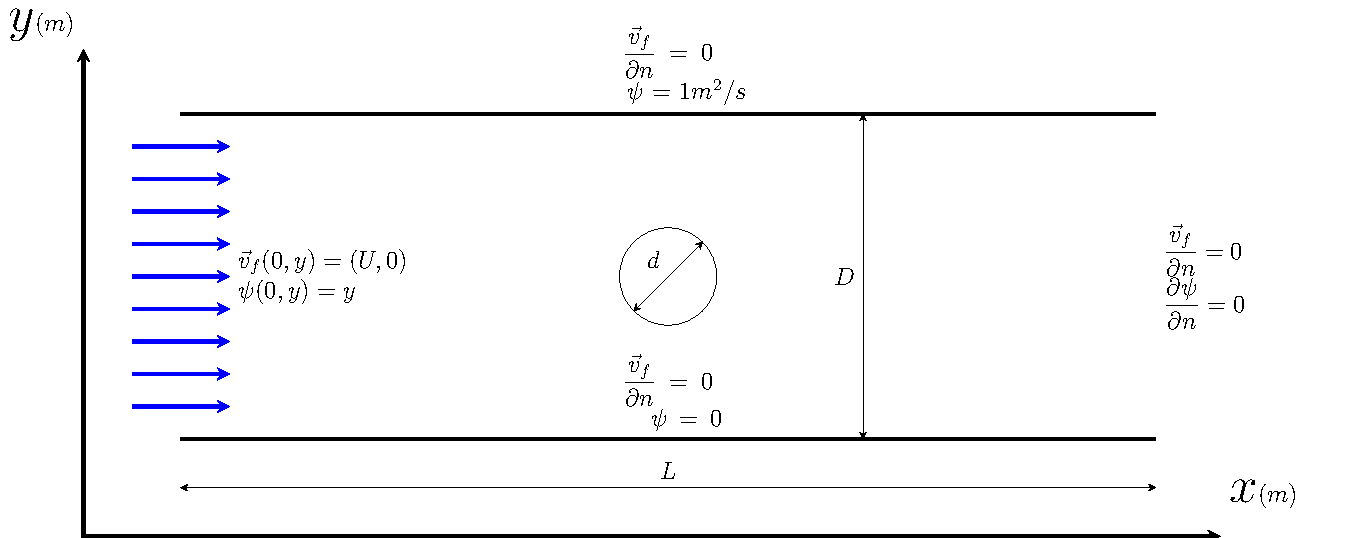
\includegraphics[height=0.38\textheight]{figure/results/Obstacle_boundary.pdf}
    } {\raggedleft \tiny Diagrama da simulação.}
  \end{figure}
  \begin{block}{Parâmetros}
    $L=8m$, $D=1m$, $d=0.3m$, $U=1m/s$, $\mu_f=50Pa.s$, $\rho_f=50kg/m^3$, $d_p=0.001m$, $\rho_p=20000kg/m^3$.
  \end{block}
\end{frame}

\begin{frame}
  \frametitle{\subsecname}
  %-
  
  \begin{figure}
    \stackunder{
      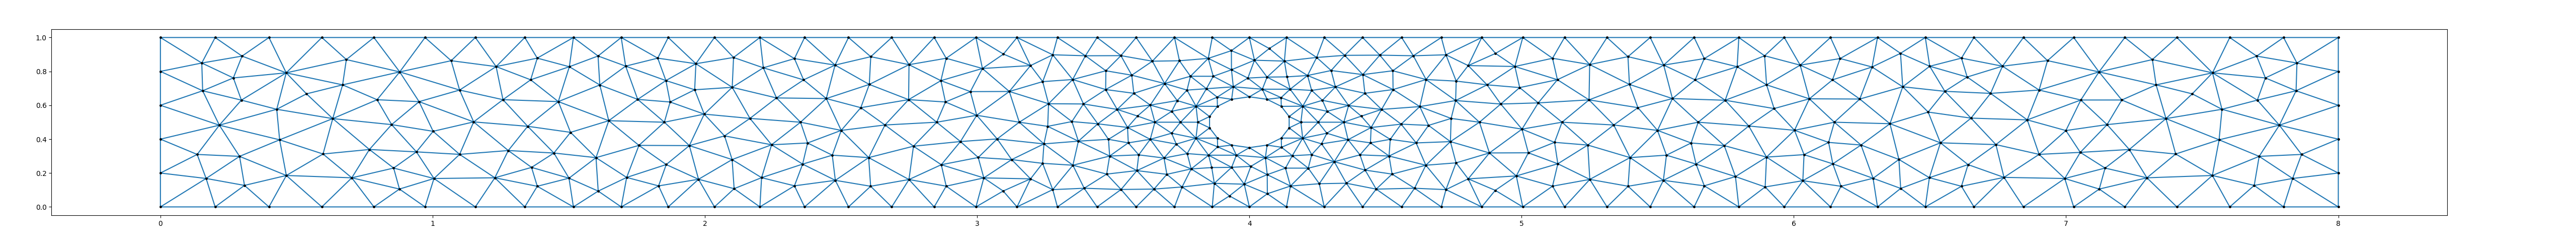
\includegraphics[width=0.98\textwidth]{figure/results/Obstacle_mesh.png}
    } {\raggedleft \tiny Malha do canal com 494 nós e 868 elementos.}
  \end{figure}
  \vspace*{-\baselineskip}\setlength\belowdisplayshortskip{0pt} % Fix display bug, empty header space
  \begin{figure}
    \stackunder{
      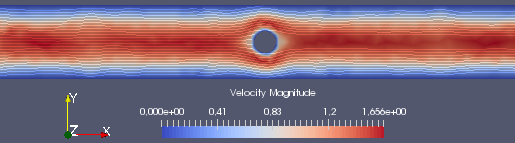
\includegraphics[height=0.28\textheight, width=0.98\textwidth]{figure/results/Obstacle_result.png}
    } {\raggedleft \tiny Campo de velocidades resultante, com $dt=0.1s$ e tempo total $t=20.0s$, realizada em torno de $1h$.}
  \end{figure}
  \vspace*{-\baselineskip}\setlength\belowdisplayshortskip{0pt} % Fix display bug, empty header space
  \begin{figure}
    \stackunder{
      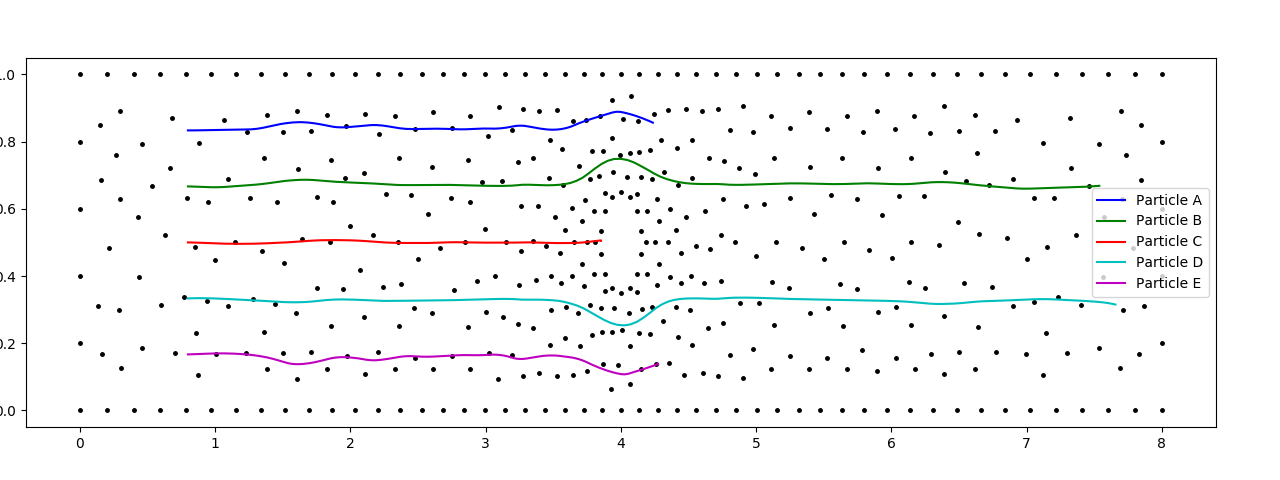
\includegraphics[height=0.28\textheight, width=0.98\textwidth]{figure/results/Obstacle_particle_trajectory.png}
    } {\raggedleft \tiny Percurso das partículas na simulação, com $dt=5E^{-5}$ e tempo total de $t=5.0s$, realizada em torno de $4h$.}
  \end{figure}
\end{frame}

%----------------------------------------------------------------------------------------------------------------------------------------------------
\subsection*{Simulação em um Canal em Degrau}
\begin{frame}
  \frametitle{\subsecname}
  %-
  
  \begin{figure}
    \stackunder{
      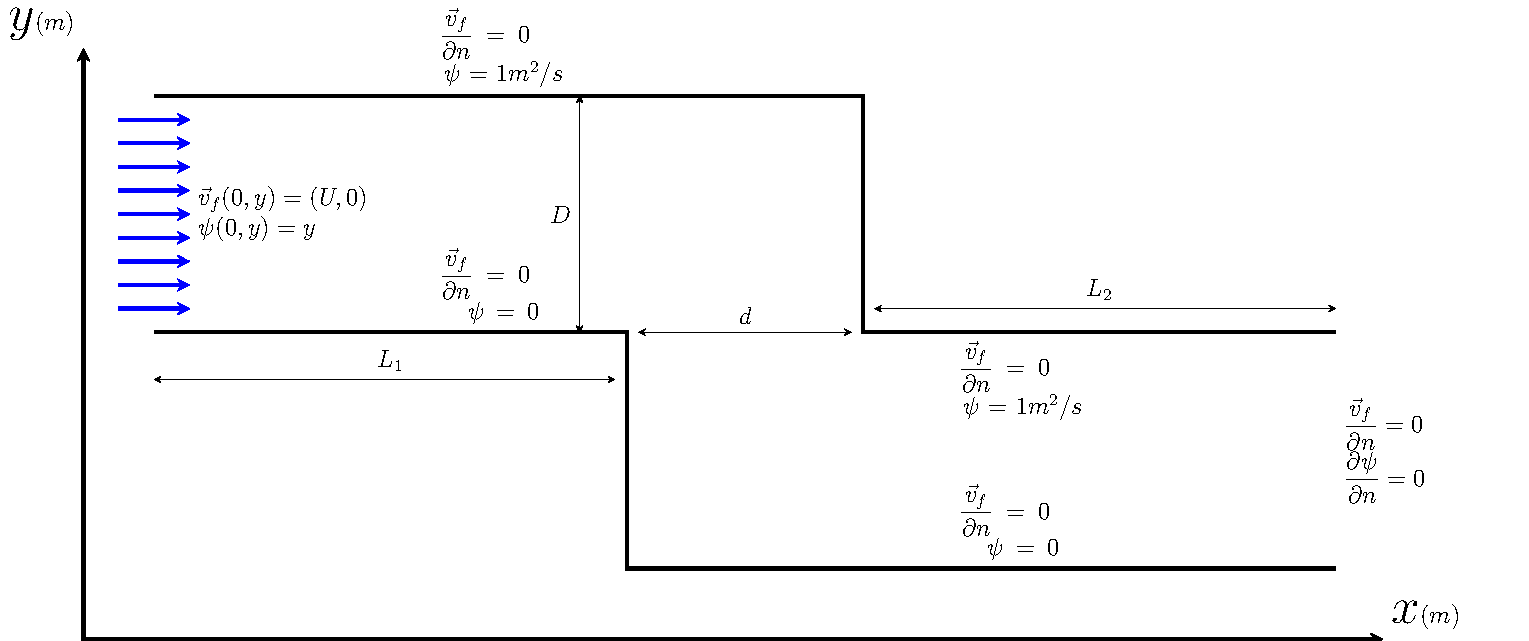
\includegraphics[height=0.38\textheight]{figure/results/Step_boundary.pdf}
    } {\raggedleft \tiny Diagrama da simulação.}
  \end{figure}
  \begin{block}{Parâmetros}
    $L_1=2m$, $L_2=2m$, $d=1m$, $D=1m$, $U=1m/s$, $\mu_f=50Pa.s$, $\rho_f=50kg/m^3$, $d_p=0.001m$, $\rho_p=20000kg/m^3$.
  \end{block}
\end{frame}

\begin{frame}
  \frametitle{\subsecname}
  %-
  
  \begin{figure}
    \stackunder{
      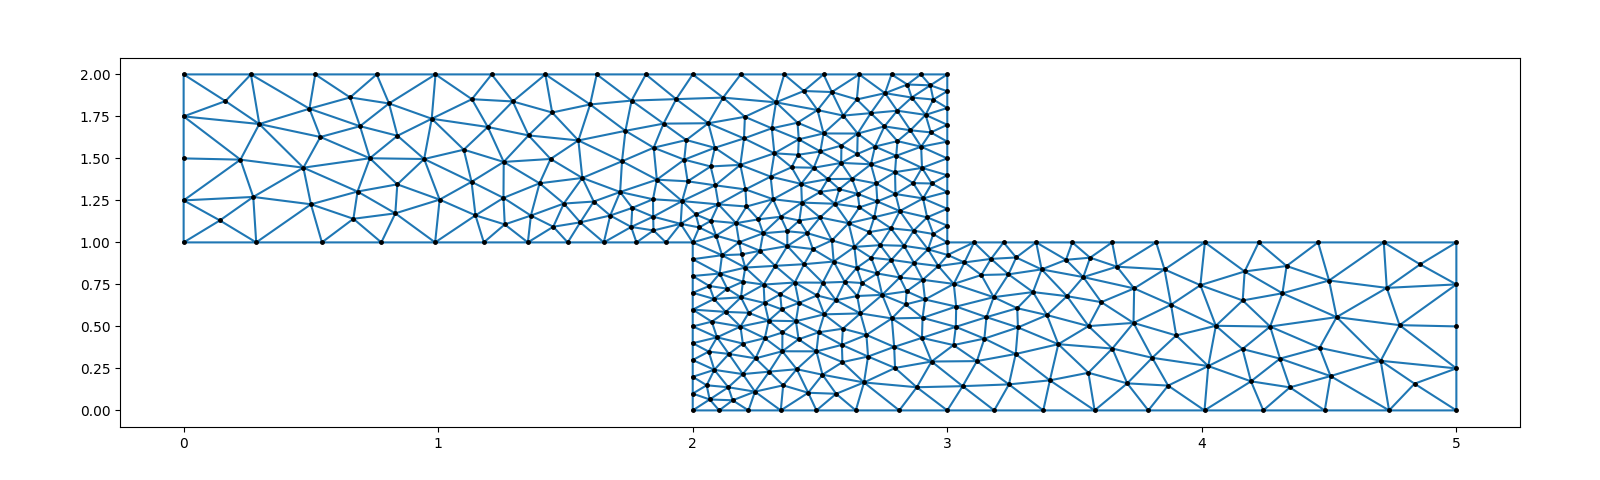
\includegraphics[width=0.98\textwidth]{figure/results/Step_mesh.png}
    } {\raggedleft \tiny Malha do canal com 380 nós e 676 elementos.}
  \end{figure}
  \vspace*{-\baselineskip}\setlength\belowdisplayshortskip{0pt} % Fix display bug, empty header space
  \begin{figure}
    \stackunder{
      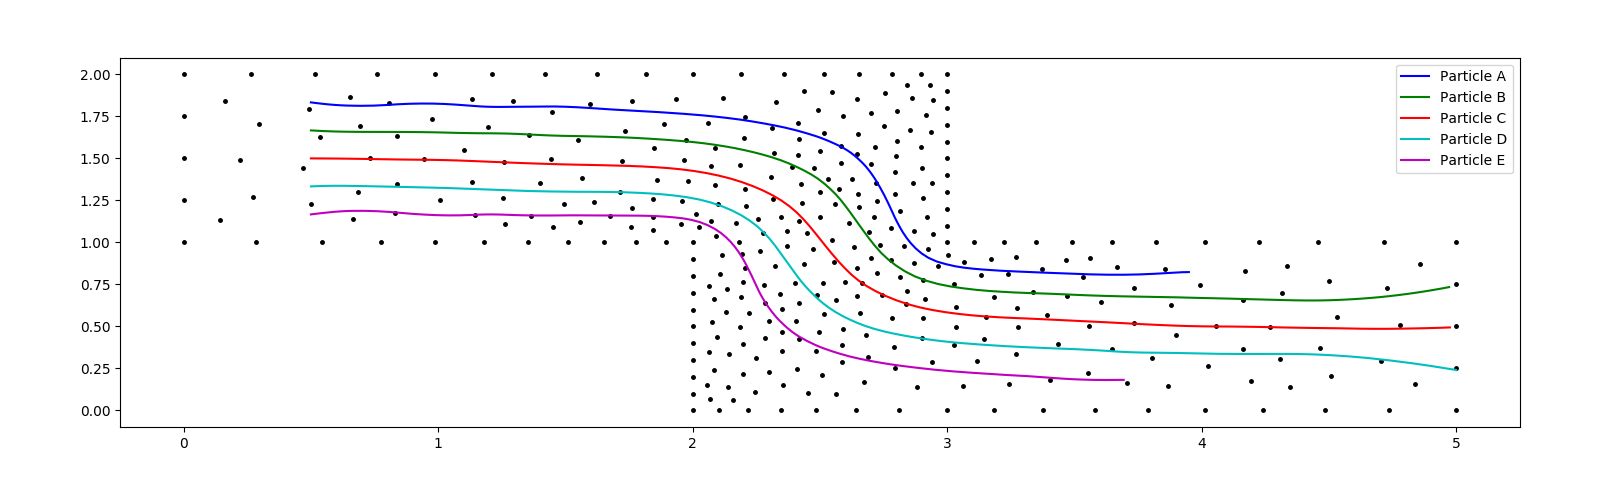
\includegraphics[height=0.28\textheight, width=0.98\textwidth]{figure/results/Step_particle_trajectory.png}
    } {\raggedleft \tiny Percurso das partículas na simulação, com $dt=5E^{-5}$ e tempo total de $t=5.0s$, realizada em torno de $4h$.}
  \end{figure}
\end{frame}


\begin{frame}
  \frametitle{\subsecname}
  %-
  \begin{figure}
    \stackunder{
      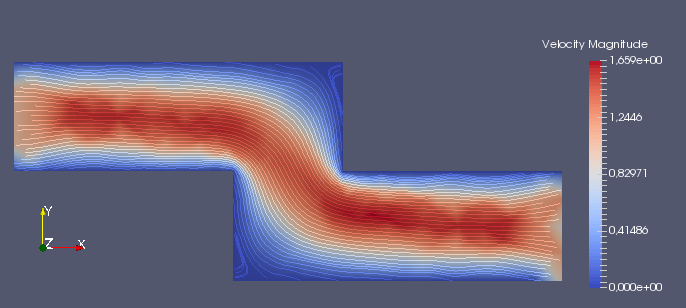
\includegraphics[width=0.98\textwidth]{figure/results/Step_result.png}
    } {\raggedleft \tiny Campo de velocidades resultante, com $dt=0.1s$ e tempo total $t=20.0s$, realizada em torno de $1h$.}
  \end{figure}
\end{frame}

%----------------------------------------------------------------------------------------------------------------------------------------------------
\subsection*{Simulação em um Canal com Restrição}
\begin{frame}
  \frametitle{\subsecname}
  %-
  
  \begin{figure}
    \stackunder{
      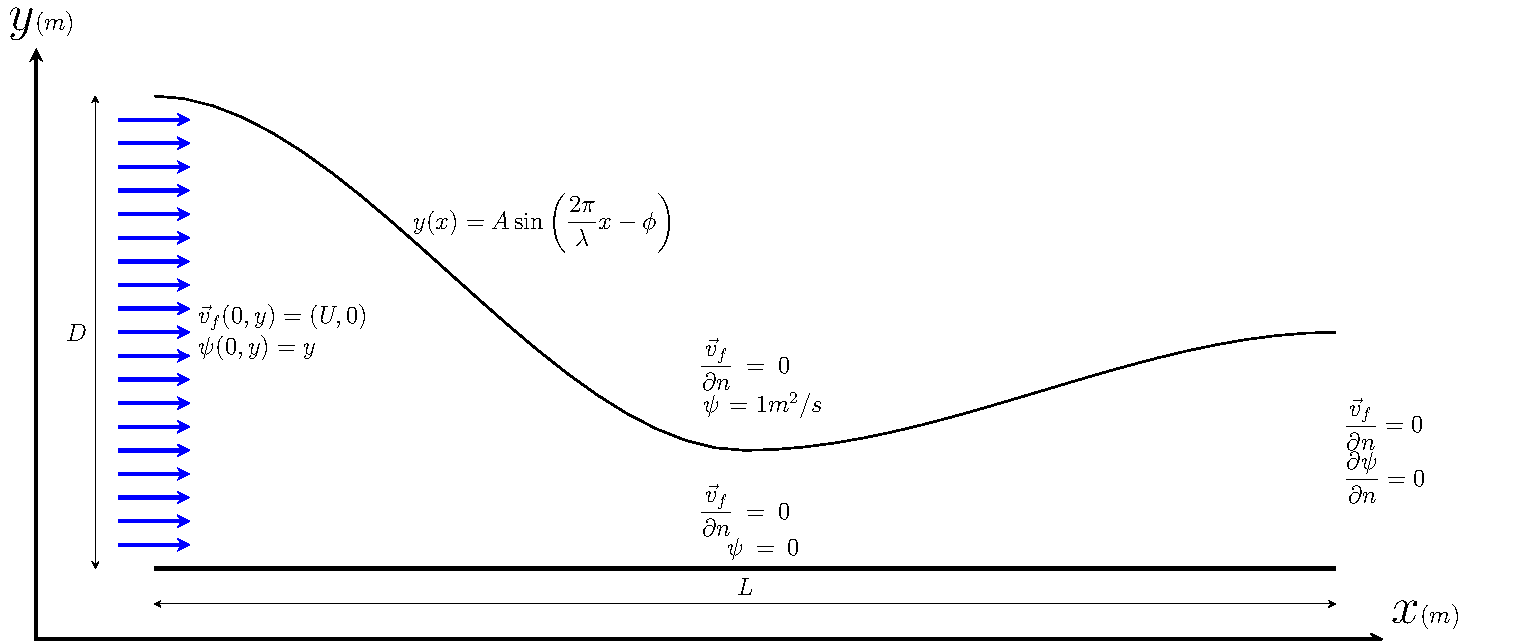
\includegraphics[height=0.38\textheight]{figure/results/Nozzle_boundary.pdf}
    } {\raggedleft \tiny Diagrama da simulação.}
  \end{figure}
  \begin{block}{Parâmetros}
    $L=8m$, $D=2m$, $A=0.004m$, $\lambda=0.0006m$, $\phi=0$, $U=1m/s$, $\mu_f=50Pa.s$, $\rho_f=50kg/m^3$, $d_p=0.001m$, $\rho_p=20000kg/m^3$.
  \end{block}
\end{frame}

\begin{frame}
  \frametitle{\subsecname}
  %-
  
  \begin{figure}
    \stackunder{
      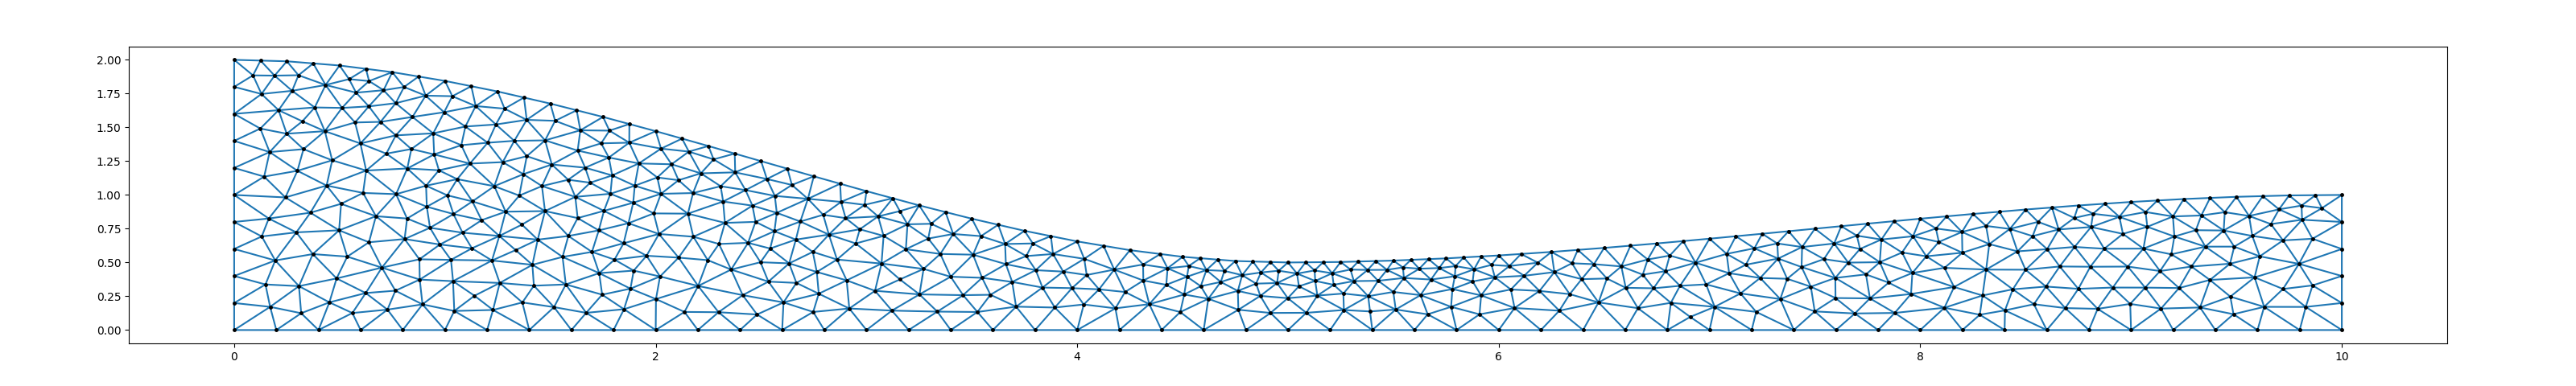
\includegraphics[height=0.15\textheight, width=0.91\textwidth]{figure/results/Nozzle_mesh.png}
    } {\raggedleft \tiny Malha do canal com 600 nós e 1047 elementos.}
  \end{figure}
  \begin{figure}
    \stackunder{
      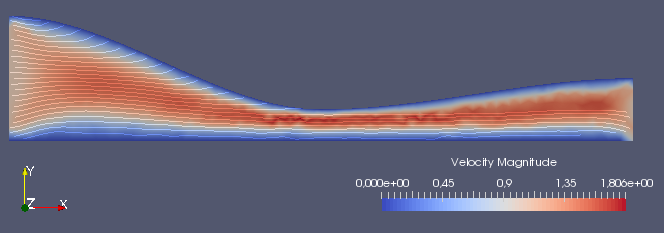
\includegraphics[height=0.28\textheight, width=0.91\textwidth]{figure/results/Nozzle_result.png}
    } {\raggedleft \tiny Campo de velocidades resultante, com $dt=0.1s$ e tempo total $t=20.0s$, realizada em torno de $2h$.}
  \end{figure}
  \vspace*{-\baselineskip}\setlength\belowdisplayshortskip{0pt} % Fix display bug, empty header space
  \begin{figure}
    \stackunder{
      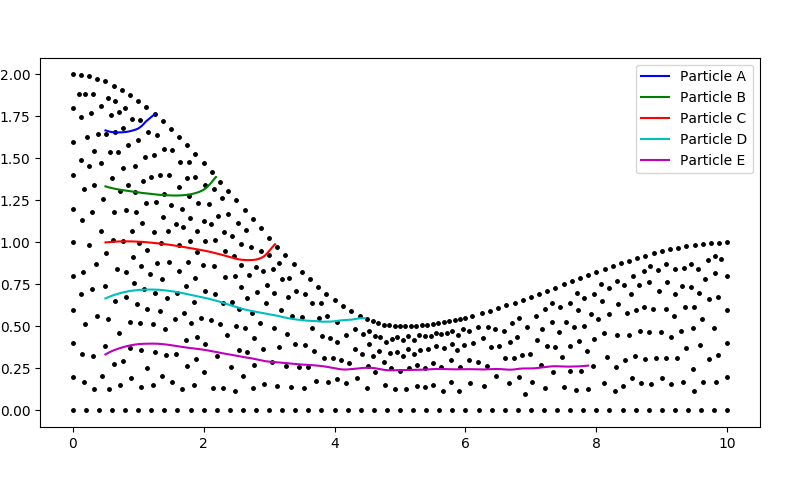
\includegraphics[height=0.28\textheight, width=0.91\textwidth]{figure/results/Nozzle_particle_trajectory.png}
    } {\raggedleft \tiny Percurso das partículas na simulação, com $dt=5E^{-5}$ e tempo total de $t=15.0s$, realizada em torno de $24h$.}
  \end{figure}
\end{frame}

%----------------------------------------------------------------------------------------------------------------------------------------------------
\subsection*{Simulações em um Impelidor}
\begin{frame}
  \frametitle{\subsecname}
  %-
  
  \vspace*{-\baselineskip}\setlength\belowdisplayshortskip{0pt} % Fix display bug, empty header space
  \begin{figure}
    \stackunder{
      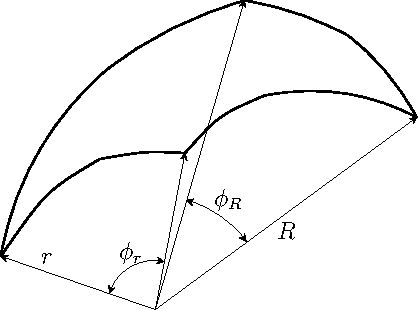
\includegraphics[height=0.538\textheight]{figure/results/Rotor_boundary.pdf}
    } {\raggedleft \tiny Diagrama da simulação.}
  \end{figure}
  \vspace*{-\baselineskip}\setlength\belowdisplayshortskip{0pt} % Fix display bug, empty header space
  \begin{block}{Parâmetros}
    $R=1m$, $r=0.75m$, $\phi_R=34^o$, $\phi_r=80^o$, $U=1m/s$, $\mu_f=50Pa.s$, $\rho_f=50kg/m^3$, $d_p,\rho_p=$por caso.
  \end{block}
\end{frame}

\begin{frame}
  \frametitle{\subsecname}
  %-
  
  \centering
  \begin{figure}
    \stackunder{
      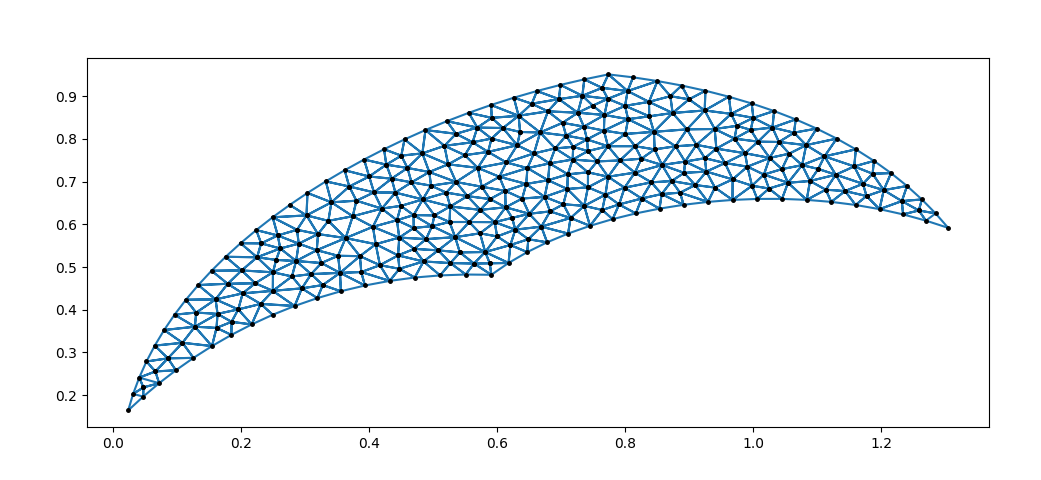
\includegraphics[height=0.28\textheight]{figure/results/Rotor_mesh.png}
    } {\raggedleft \tiny Malha do canal com 531 nós e 1058 elementos.}
  \end{figure}
  \vspace*{-\baselineskip}\setlength\belowdisplayshortskip{0pt} % Fix display bug, empty header space
  \begin{figure}
      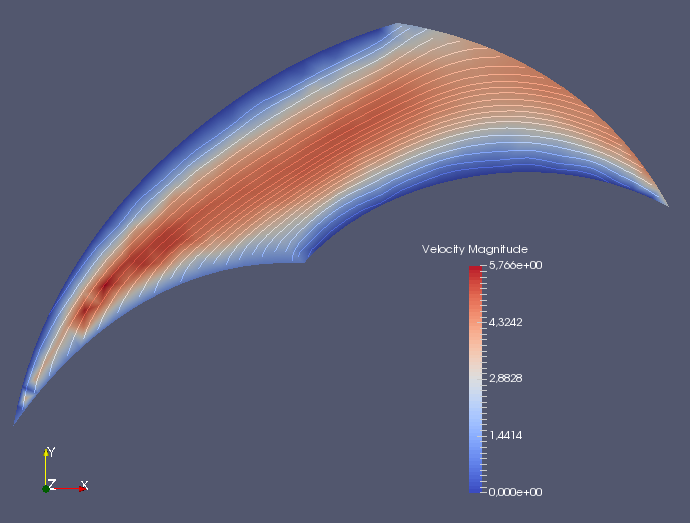
\includegraphics[height=0.38\textheight]{figure/results/Rotor_result.png}
  \end{figure}
  \raggedleft \tiny Campo de velocidades resultante, com $dt=0.1s$ e tempo total $t=20.0s$, realizada em torno de $2h$.
\end{frame}
  
\begin{frame}
  \frametitle{\subsecname}
  \centering
  \begin{minipage}{.48\textwidth}
%     \centering
    \begin{block}{}
    \footnotesize
      Simulações dos percursos das partículas efetuadas com $dt=5E^{-5}$ e tempo total de $t=5.0s$, realizadas em torno de $12h$.
    \end{block}
  \end{minipage}
  \hfill
  \begin{minipage}{.48\textwidth}
%     \centering
    \begin{figure}
      \stackunder{
	\includegraphics[height=0.38\textheight,width=\textwidth]{figure/results/Rotor_particle_trajectory_gold.png}
      } {\raggedleft \tiny Partículas de ouro, $d_p=1E^{-3}m$ e $\rho_{Au}=2E^{4}kg/m^3$.}
    \end{figure}
  \end{minipage}
  
  \begin{minipage}{.48\textwidth}
    \begin{figure}
      \stackunder{
	\includegraphics[height=0.38\textheight,width=\textwidth]{figure/results/Rotor_particle_trajectory_iron.png}
      } {\raggedleft \tiny Partículas de ferro, $d_p=1E^{-3}m$ e $\rho_{Fe}=7.3E^{3}kg/m^3$.}
    \end{figure}
  \end{minipage}
  \hfill
  \begin{minipage}{.48\textwidth}
    \begin{figure}
      \stackunder{
	\includegraphics[height=0.38\textheight,width=\textwidth]{figure/results/Rotor_particle_trajectory_sand.png}
      } {\raggedleft \tiny Partículas de areia, $d_p=5E^{-4}m$ e $\rho_p=1.6E^{3}kg/m^3$.}
    \end{figure}
  \end{minipage}
\end{frame}

%----------------------------------------------------------------------------------------------------------------------------------------------------
\section*{}
\begin{frame}
  \frametitle{Conclusão}
  %-Plataforma de estudos de escoamento multifásico 2D em geometrias complexas através do MEF.
  
  \centering
  \fontsize{10pt}{7.2}\selectfont
  \begin{block}{Conclusões}
    \begin{itemize}
      \item A linguagem Python é uma excelente ferramenta para criar simuladores, ela permite realizar cálculos complexos rapidamente.
      \item A o modelo e a biblioteca representam bem o fenômeno esperado.
      \item Para os casos estudados, força de arrasto possuí a maior contribuição ao movimento.
      \item Embora a biblioteca utilize o armazenamento de matrizes esparsas, as simulações levam bastante tempo.
    \end{itemize}
  \end{block}
  
  \begin{block}{Pontos fracos}
    \begin{itemize}
      \item O simulador requer um grande esforço computacional.
      \item Não foi implementada a funcionalidade de \textit{multithreading} na biblioteca.
      \item Restrição de uso para valores de Reynolds $<$ 1.
    \end{itemize}
  \end{block}
\end{frame}

%----------------------------------------------------------------------------------------------------------------------------------------------------
% Bibliografia
%----------------------------------------------------------------------------------------------------------------------------------------------------

% \begin{frame}
%   \frametitle{Bibliografia}
%   \footnotesize{
%     \todo[inline]{Fazer bibliografia}
%     \begin{thebibliography}{99} % Beamer does not support BibTeX so references must be inserted manually as below
% 
%       \bibitem[biezuner]{p1} R.J. Biezuner (2007)
%       \newblock Métodos Numéricos para Equações Parciais Elípticas
%       \newblock \emph{Notas de Aula}
% 
%       \bibitem[fortuna]{p1} A.O. Fortuna (2000)
%       \newblock Técnicas Computacionais para Dinâmica dos Fluidos: Conceitos Básicos e Aplicações
%       \newblock \emph{Edusp}
% 
%       \bibitem[leveque]{p1} R.J. LeVeque (2007)
%       \newblock Finite Difference Methods for Ordinary and Partial Differential Equations. Steady-State and Time-Dependant Problems
%       \newblock \emph{SIAM}
% 
%       \bibitem[biezuner]{p1} J.R. Rodrigues (2015)
%       \newblock Introdução à Simulação de Reservatórios Petrolíferos
%       \newblock \emph{Programa de Verão LNCC}
%     \end{thebibliography}
%   }
% \end{frame}

%----------------------------------------------------------------------------------------------------------------------------------------------------
% Agradecimentos
%----------------------------------------------------------------------------------------------------------------------------------------------------
\section*{}
\begin{frame}
  \frametitle{Agradecimentos}
  \centering
  \begin{tikzpicture}
    \node[inner sep=0cm] (gesar) at (0,0){
      \includegraphics[width=0.2\textwidth]{figure/gesar-logo-new.png}};
    \node[inner sep=0cm] (uerj) at (4,0){
      \includegraphics[width=0.2\textwidth]{figure/UERJ.png}};
    \node[inner sep=0cm] (fen) at (8,0){
      \includegraphics[width=0.2\textwidth]{figure/fen-new.png}};
  \end{tikzpicture}
  \Huge{\centerline{Muito Obrigado!}}
\end{frame}

%----------------------------------------------------------------------------------------

\end{document}
% Reduzir numero de slides, usar mais de uma figura por slide